{\it Author's note}: As this is a continuation of the first part of this paper
\cite{WebcohI}, we will use notation and constructions from that paper
without additional reference or comment. 

\section{(Re)introduction}
\label{sec:reintroduction}

In \cite{WebcohI,WebGT, WebSD}, we developed a general theory of Coulomb
branches from an algebraic perspective.  We showed that the Coulomb
branch algebra itself, its extended category (of line operators) and
various related algebras, such as the non-commutative resolution
constructed through quantization by Bezrukavnikov and Kaledin
\cite{BKpos,KalDEQ, BezNon} and the category controlling their
Gelfand-Tsetlin modules all have explicit combinatorial descriptions
based on the  structure of their weight spaces.  In this sequel to
these papers, we focus in on understanding this construction in the
quiver gauge case, especially on the non-commutative resolution and
corresponding geometric constructions with coherent sheaves.
Applications to the representation theory of quantum Coulomb branches
in characteristic 0 have already been covered extensively in
\cite{KTWWY2, WebGT, Webalt}, so we will only discuss these in
passing.

At the root of this perspective is a description of the Coulomb branch
algebra as paths in the space $T_{\R}/W$, the quotient of the compact
torus of the gauge group $G$ modulo the Weyl group $W$, modulo certain
relations (see \cite[(2.5a--c)]{WebSD}).  In the case
of $GL_n$, this space can be identified with the configuration of $n$
points on the circle $\R/\Z$ (allowing collisions), and thus a path in this space with a
diagram drawn on the cylinder.


Fix a quiver $\gls{quiver}$
with vertex set ${\gls{vertex}}$, and dimension vectors $\gls{Bv},\gls{Bw}\colon {\vertex}\to
\Z_{\geq 0}$ for this quiver.  We should emphasize that we do allow edge loops.   By a {\bf quiver gauge theory} we mean
the one attached to the gauge group and matter $(G,V)$ given by: 
\begin{equation}
\gls{G}=\prod GL(\C^{v_i})\qquad \gls{V}=\Big(\bigoplus_{i\to j}
\Hom(\C^{v_i},\C^{v_j})\Big)\bigoplus \Big(\bigoplus_{i\in {\vertex}}
  \Hom(\C^{w_i},\C^{v_i}) \Big),\label{eq:quiver-gauge2}
\end{equation}
As described above, we can think of a path in $T_{\R}/W$ as a path in
a labeled configuration space where $v_i$ points have label $i$, that
is, as a string diagram on the cylinder where strands are labeled by
points in the Dynkin diagram.  When we translate the relations
\cite[(2.5a--c)]{WebSD} into this framework, they suddenly become very
familiar to any one used to categorification: those of the KLR
algebra, as presented in \cite{KLII}.  The author and his
collaborators exploited this in \cite{KTWWY2} to study the
representation theory of shfited Yangians, but by taking a more
geometric perspective, we can apply the same idea to categories of
coherent sheaves.

Thus our main result is a description of a tilting generator on the
resolved Coulomb branch for affine type A gauge theories, i.e. those
with cyclic or linear quivers.  The most interesting examples of these
are resolved Slodowy slices (or more generally, S3 varieties) for a linear
quiver and the Hilbert scheme of points on $\C^2$ (for more generally,
the resolved Kleinian singularity $\C^2/\Z/\ell\Z$).  
\begin{itheorem}
  If $\gls{Coulomb}$ is the Coulomb branch of an affine type $A$ quiver gauge
  theory, and $\gls{tM}$ a BFN resolution, then:
  \begin{enumerate}
  \item the homogeneous coordinate ring of $\gls{tM}$ is an algebra of
    twisted cylindrical KLR diagrams, module local relations.
  \item The variety $ \gls{tM}$ admits a tilting generator $\mathcal{T}$,
    described as an explicit module over the homogenous coordinate
    ring, such that $\End(\mathcal{T})$ is a cylindrical wKLR algebra.
  \item The wall-crossing functors relating different tilting
    generators are given by tensor product with explicit bimodules,
    modeled on the braiding functors of \cite[\S 6]{Webmerged}; more
    generally, the Schober connected to these functors can constructed
    using the representation theory of related algebras.
  \end{enumerate}
\end{itheorem}
Aside from making explicit a construction that otherwise requires some
rather challenging techniques, it's generally believed that the
algebras $\End(\mathcal{T})$ are Koszul; we hope that this can be
proved geometrically, much as similar results have been proven for
usual weighted wKLR algebras.  Other possible applications include
studying Bezrukavnikov and Okounkov's conjecture relating
wall-crossing functors to quantum cohomology and generalizing Anno and
Nandakumar's work on affine tangles in 2-block Springer fibers to more
general actions of webs.  

\section{Diagrams for quiver gauge theories}


First, we note some basic facts about quiver gauge theories.  In this case, the group $\gls{No}=N_{GL(V)}(G)$ is generated by $\gls{G}$, the product
$GL(\C^{\glslink{Bw}{w_i}})$ acting by precomposition in the obvious way, and by
$GL(\C^{\chi_{i,j}})$ where $\chi_{i,j}$ is the number of edges
$i\to j$, acting by taking linear combinations of the maps along these
edges, i.e. via the isomorphism
\[\bigoplus_{i\to j}\Hom(\C^{\glslink{Bv}{v_i}},\C^{\glslink{Bv}{v_j}})\cong \bigoplus_{(i,j)\in {\vertex}}
  \Hom(\C^{\glslink{Bv}{v_i}},\C^{\glslink{Bv}{v_j}})\otimes \C^{\chi_{i,j}}.\]

For simplicity, we'll assume that $\gls{delta}=\frac{1}{2}$ (and so in
\gls{pthroot} conventions, we have $\gls{delta}=\frac{1}{2p}$).

\subsection{Unrolled diagrams}
\label{sec:diagr-descr}

In the case of a quiver gauge theory, the extended BFN category has
a more graphical description.  Let us first discuss a little how the
constructions of \cite{WebcohI} can be interpreted here.

The space $\gls{ft}_{\R}$ in this case is naturally isomorphic to
$\bigoplus_{i\in {\gls{vertex}}}\R^{\glslink{Bv}{v_i}}$, using the usual coordinates on diagonal
matrices.  These coordinates are given by $z_{i,k}=\ep_{i,k}$ with $i\in {\gls{vertex}},
k=1,\dots, v_i$
ranging over the weights of the natural representation of
$GL(\mathbb{C}^{v_i})$.

In these terms, the unrolled arrangments defined in Section
\ref{sec:extended} are given by the unrolled root hyperplanes
$\{\alpha(\acham)=n\mid n\in\Z\}$ of the form:\newseq
\[\subeqn z_{i,k}-z_{i,m}=n\qquad \text{ for all }k\neq m\in [1,\glslink{Bv}{v_i}], n\in \Z,\label{eq:unroll-root}\] and the unrolled
matter hyperplanes $\{\varphi_i^{\operatorname{mid}}(\acham)=n\mid n\in
\Z\}$  of the form:
\begin{align*}\subeqn\label{eq:unroll-matter1}
z_{j,k}-z_{i,m}&=n-\frac{1}{2}\qquad \text{ for all edges } i\to j,
  \text{ for all } k\in [1,\glslink{Bv}{v_j}], m\in [1,\glslink{Bv}{v_i}], n\in \Z\\
\subeqn z_{i,m}&=n-\frac{1}{2}\qquad \text{ for all } i\in {\vertex}, m\in [1,\glslink{Bv}{v_i}], n\in \Z\label{eq:unroll-matter2   }
\end{align*}

We can decompose a path $\pi \colon  [0,1]\to \ft$ into a
$\glslink{Bv}{v_i}$-tuple of paths $\pi_{i,k}$ for each $i\in {\vertex}$.  We can visualize
this by superimposing the graphs of these paths (though we will use
the opposite convention from calculus class, using the $y$-axis for
the independent variable and the $x$-axis for the dependent).  That
is, we consider the path $t\mapsto (\pi_{i,k}(t),t)$ landing in
$\R\times [0,1]$.

We cross root hyperplanes when two of these paths for the same element
of ${\vertex}$ are integer distance
from each other, and matter hyperplanes when either the $x$-value or
the distance between two paths corresponding to adjacent nodes in ${\vertex}$
differ by an element of $\Z-\frac{1}{2}$.

It's thus convenient to label the points $(\pi_{i,k}(t)+n,t)$ for
$n\in \Z$ with ``partner'' strands and those for $n\in \Z-\frac{1}{2}$ with ``ghost'' strands so that we can see when these
crossings occur.  We'll label the strand corresponding to $n$ with $i;n$.  We'll draw partners as solid lines,
and ghosts as dashed lines.  We'll also draw in dashed
lines at $x=n$ for $n\in \Z-\frac{1}{2}$, which we'll label with
$\infty;n$.


There's an obvious action of the affine Weyl group on the set of such
paths with the finite Weyl group acts on paths by permutation of
the second indices in $\pi_{i,k}$, and the translations act by
translations $\pi_{i.k}(t)\mapsto \pi_{i,k}(t)+n_{i,k}$ for integers
$n_{i,k}$.  This leaves the collections of the original curves and
their partners unchanged, just changing the indices and which curves
are partners, and which are originals. Thus, we can visualize the
action of an affine Weyl group element by changing the labels
accordingly at some fixed value of $y=a$.  The equations
(\ref{eq:conjugate2}) and (\ref{eq:psiconjugate}) assure that the
result does not depend on the value of $a$.  

We can also visualize the action of $\glslink{S}{S_h}$ by identifying the weights
$\ep_{i,k}$ with a dot on the corresponding path, at the top for
multiplying at the left and at the bottom for multiplication on the
right.  It will be useful to also draw dots on partner strands with
label $i;n$, which we will associate to $\ep_{i,k}+nh$.  This likewise
assures that inserting an element of the affine Weyl group above or
below a dot will give the same answer, by equation (\ref{eq:dot-commute}).

Thus, the morphisms in $\gls{scrB}$ can all be expressed as one of these diagrams.  More precisely:
\begin{definition}
  An {\bf unrolled diagram} is a collection of paths in $\R\times
  [0,1]$ of the form $\{ (\pi_{i,k}(t)+n,t) \mid t\in [0,1]\}$ for
  $n\in \Z$ for some piecewise 
  smooth map $\pi_{i,k}\colon [0,1]\to \R$.  At a finite number of
  values $t_1,\dots, t_k$, we apply an elements $w_1,\dots, w_k\in
  \widehat{W}$ to the labels on the curves and their partners, which can
  create a discontinuity in the function $ \pi_{i,k}$, but we assume
  that the resulting curves are still smooth and simply change
  labeling.  We'll draw one of these changes as a squiggly green line.

  We also add
  ghost strands 
  at $\{ (\pi_{i,k}(t)+n-\frac{1}{2},t) \mid t\in [0,1]\}$ and at $\{
  (n-\frac{1}{2},t) \mid t\in [0,1]\}$ for all $n\in \Z$, which we draw as dashed. Each curve is labeled with the element $i\in {\gls{vertex}}$ and decorated with
  finitely many dots.

  The diagram must be locally of the
  form \begin{equation}\label{eq:unrolled-possible}
    \begin{tikzpicture}[baseline,scale=.9]
      
  \draw[very thick] (-12,0) +(-1,-1) -- +(1,1);
 
  \draw[very thick, dashed](-12,0) +(1,-1) -- +(-1,1);
 


  \draw[very thick, dashed] (-8,0) +(-1,-1) -- +(1,1);
 
  \draw[very thick](-8,0) +(1,-1) -- +(-1,1);
 

  \draw[very thick] (-4,0) +(-1,-1) -- +(1,1);
   % node[below,at start] {$i$};
  \draw[very thick](-4,0) +(1,-1) -- +(-1,1);
  %  node[below,at start] {$j$};

%\draw[very thick] (0,0) +(0,-1) -- +(0,1)
%node[below, at start]{$i$};
%\fill (0,0) circle (5pt);


  \draw[very thick](-1,0) +(0,-1) --  node
  [midway,circle,fill=black,inner sep=2pt]{}
  +(0,1);


  \draw[very thick](1.5,0) +(0,-1) -- 
  +(0,1);
    \draw[weyl](1.5,0) +(-.5,0) -- 
  +(.5,0);
\end{tikzpicture}
\end{equation}
That is, there are no tangencies, triple crossings or dots on
crossings.  The curves (including ghosts) must
meet the circles at
$y=0$ and $y=1$ at distinct points. We consider these
diagrams 
up to isotopy preserving the conditions above.
\end{definition}
We'll draw an example below; lacking infinitely wide
paper, we can only draw part of the diagram.
\begin{equation} \label{eq:unroll-example}
       \tikz[very thick,xscale=1.5,baseline]{
           \draw (.8 ,-1) to node[below,at start, scale=.8]{$i;0$}(-.3,1);
           \draw (-.8 ,-1) to node[above, at end, scale=.8]{$j;-1$} (.3,1);
               \draw (-1.2 ,-1) to  node[below,at start, scale=.8]{$i;-1$} (-2.3,1);
               \draw (-2.8 ,-1) to node[above, at end, scale=.8]{$j;-2$}  (-1.7,1);
               \draw (1.2 ,-1) to node[above, at end, scale=.8]{$j;0$}  (2.3,1);
        \draw (2.8 ,-1) to  node[below,at start, scale=.8]{$i;1$} (1.7,1);
        \draw[dashed] (-.2,-1) -- node[below,at start, scale=.8]{$i;-\nicefrac{1}{2}$} (-1.3,1);
        \draw[dashed] (.2,-1) --  node[above, at end, scale=.8]{$j;-\nicefrac{1}{2}$}  (1.3,1);
        \draw[dashed] (-.7,1) -- node[above, at start, scale=.8]{$j;-1\nicefrac{1}{2}$}  (-1.8,-1);
        \draw[dashed] (.7,1) -- node[below,at end,
        scale=.8]{$i;\nicefrac{1}{2}$} (1.8,-1);
        \draw[dashed] (-2.2,-1) -- node[below,at start, scale=.8]{$i;-1\nicefrac{1}{2}$} (-3.3,1);
        \draw[dashed] (2.2,-1) --  node[above, at end, scale=.8]{$j;\nicefrac{1}{2}$}  (3.3,1);
        \draw[dashed] (-2.7,1) -- node[above, at start, scale=.8]{$j;-2\nicefrac{1}{2}$}  (-3.8,-1);
        \draw[dashed] (2.7,1) -- node[below,at end,
        scale=.8]{$i;1\nicefrac{1}{2}$} (3.8,-1);
        \node at (4.2,0){$\cdots$};
         \node at (-4.2,0){$\cdots$};
        }
\end{equation}
%\begin{equation*} 
 %      \tikz[very thick,xscale=1.5,baseline]{
 %          \draw[dashed] (-1 ,-1) to(.8,1);
 %       \draw (-.7 ,-1) to (-.1,1);
 %       \draw[dashed] (.3 ,-1) to (.9,1);     
 %       \draw (0 ,-1) to (1,0.1111111111);
 %           \draw (-1 ,0.1111111111) to (-.2,1);
 %       \draw[dashed] (.3 ,-1) to (.9,1); }
%\end{equation*}


We can associate a morphism $\mathbbm{r}_D$ to an unrolled diagram via
the rules we have already discussed.  The diagram $D$ corresponds to a
map $[0,1]\to \ft_{\R}$,  and we can define $\pi$ by adding the flavor
$\gls{flav}$ to this path to obtain one in $\ft_{1,\R}$.  
\begin{definition}\hfill
  \begin{enumerate}
  \item Given an unrolled diagram $D$ with no dots, let
    $\mathbbm{r}_D$ be the morphism $\mathbbm{r}_\pi$ for the
    corresponding path.
  \item
    Given an unrolled diagram with all
    $\pi_{i,k}$'s constant, and one dot on the strand at
    $(\pi_{i,k}+n,t)$, we let $\mathbbm{r}_D$ be multiplication by
    $\ep_{i,k}+nh$.
\item   Given an unrolled diagram with no dots, and a single
  relabeling by $w\in \widehat{W}$, we let $\mathbbm{r}_D=y_w$.
  \end{enumerate}
Any other diagram can be written as a composition of these, and we
define $\mathbbm{r}_D$ to be the composition of the corresponding morphisms.
\end{definition}

This associates a morphism to a diagram, and since we hit all the
generators of the category $\gls{scrB}$, every morphism is a sum of
$\mathbbm{r}_D$'s.  However, this description is redundant, since
there are relations between these generators. 

\newseq
 All our relations can be described locally in terms of unrolled
 diagrams.  In order to write these relations in a consistent way, we
 need to adopt the ``dot migration'' convention for interpreting dots
 on partner strands:
\begin{equation*}\label{eq:dot-migration}\subeqn
    \begin{tikzpicture}[very thick,baseline,scale=.9]       \draw (1,0)
      +(1,-1) -- +(1,1) node[below,at start,scale=.8]{$i;n$};  \fill (2,0) circle (3.5pt);\node at (.5,0){$\cdots$}; \draw (0,0)
      +(-1,-1) -- +(-1,1) node[below,at start]{$i$};  
    \end{tikzpicture}=\:\begin{tikzpicture}[very thick,baseline,scale=.9]       \draw (1,0)
      +(1,-1) -- +(1,1) node[below,at start,scale=.8]{$i;n$};  \fill (-1,0) circle (3.5pt);\node at (.5,0){$\cdots$}; \draw (0,0)
      +(-1,-1) -- +(-1,1) node[below,at start]{$i$};  
    \end{tikzpicture}+nh\:\begin{tikzpicture}[very thick,baseline,scale=.9]       \draw (1,0)
      +(1,-1) -- +(1,1) node[below,at start,scale=.8]{$i;n$}; \node at (.5,0){$\cdots$}; \draw (0,0)
      +(-1,-1) -- +(-1,1) node[below,at start]{$i$};  
    \end{tikzpicture}
  \end{equation*}
 The fact that isotopy leaves $\mathbbm{r}_D$ invariant is a
combination of relations (\ref{eq:dot-commute}) and the ``boring''
cases of
(\ref{eq:wall-cross1},\ref{eq:psi},\ref{eq:psipoly},\ref{eq:triple})
where the portions of diagrams commuting past each other are distant
in $\R$.  As discussed before,
(\ref{eq:weyl1},\ref{eq:conjugate2},\ref{eq:weyl2},\ref{eq:psiconjugate})
imply that green lines can isotope past all crossings and dots, and
(\ref{eq:coweight2}) that green lines can merge by multiplying their
labels.  
\begin{equation*}\label{eq:antipodal-possible}\subeqn
    \begin{tikzpicture}[baseline,scale=.9]
        \draw[very thick] (-4,0) +(-1,-1) -- +(1,1);
   % node[below,at start] {$i$};
  \draw[very thick](-4,0) +(1,-1) -- +(-1,1);
  %  node[below,at start] {$j$};
  \draw[weyl] (-4,.5) +(1.5,0) -- +(-1.5,0);
  \end{tikzpicture}=   \begin{tikzpicture}[baseline,scale=.9]
        \draw[very thick] (-4,0) +(-1,-1) -- +(1,1);
   % node[below,at start] {$i$};
  \draw[very thick](-4,0) +(1,-1) -- +(-1,1);
  %  node[below,at start] {$j$};
  \draw[weyl] (-4,-.5) +(1.5,0) -- +(-1.5,0);
  \end{tikzpicture}\qquad \qquad 
   \begin{tikzpicture}[baseline,scale=.9]
  \draw[very thick](-1,0) +(0,-1) --  node
  [midway,circle,fill=black,inner sep=2pt]{}
  +(0,1);
  \draw[weyl] (-1,.5) +(0.5,0) -- +(-0.5,0);
\end{tikzpicture}=  \begin{tikzpicture}[baseline,scale=.9]
  \draw[very thick](-1,0) +(0,-1) --  node
  [midway,circle,fill=black,inner sep=2pt]{}
  +(0,1);
  \draw[weyl] (-1,-.5) +(0.5,0) -- +(-0.5,0);
\end{tikzpicture}
\end{equation*}
\begin{equation*}
      \begin{tikzpicture}[baseline,scale=.9]
      
  \draw[very thick] (-12,0) +(-1,-1) -- +(1,1);
 
  \draw[very thick, dashed](-12,0) +(1,-1) -- +(-1,1);
 
  \draw[weyl] (-12,.5) +(1.5,0) -- +(-1.5,0);
\end{tikzpicture}=      \begin{tikzpicture}[baseline,scale=.9]
      
  \draw[very thick] (-12,0) +(-1,-1) -- +(1,1);
 
  \draw[very thick, dashed](-12,0) +(1,-1) -- +(-1,1);
 
  \draw[weyl] (-12,-.5) +(1.5,0) -- +(-1.5,0);
\end{tikzpicture}\qquad 
\begin{tikzpicture}[baseline,scale=.9]

  \draw[very thick, dashed] (-8,0) +(-1,-1) -- +(1,1);
 
  \draw[very thick](-8,0) +(1,-1) -- +(-1,1);
  
  \draw[weyl] (-8,.5) +(1.5,0) -- +(-1.5,0);
\end{tikzpicture}=\begin{tikzpicture}[baseline,scale=.9]

  \draw[very thick, dashed] (-8,0) +(-1,-1) -- +(1,1);
 
  \draw[very thick](-8,0) +(1,-1) -- +(-1,1);
  
  \draw[weyl] (-8,-.5) +(1.5,0) -- +(-1.5,0);
\end{tikzpicture}
\end{equation*}
These relations make the need for the rule (\ref{eq:dot-migration}) clear.

The relation 
(\ref{eq:dot-commute}) implies that dots can commute past strands with a
different label or their partners, or past all ghosts:
\begin{equation*}\subeqn\label{b-first-QH}
    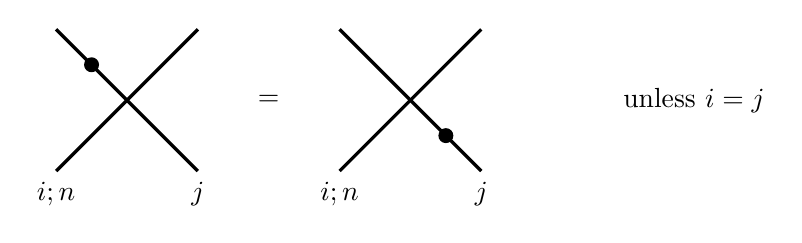
\begin{tikzpicture}[scale=.9,baseline]
      \draw[very thick](-4,0) +(-1,-1) -- +(1,1) node[below,at start]
      {$i;n$}; \draw[very thick](-4,0) +(1,-1) -- +(-1,1) node[below,at
      start] {$j$}; \fill (-4.5,.5) circle (3pt);
      % \draw[very thick] (0,0) +(0,-1) -- +(0,1) node[below, at
      % start]{$i$}; \fill (0,0) circle (5pt);
      \node at (-2,0){=}; \draw[very thick](0,0) +(-1,-1) -- +(1,1)
      node[below,at start] {$i;n$}; \draw[very thick](0,0) +(1,-1) --
      +(-1,1) node[below,at start] {$j$}; \fill (.5,-.5) circle (3pt);
      \node at (4,0){unless $i=j$};
    \end{tikzpicture}
  \end{equation*}
\begin{equation*}\subeqn\label{b-second-QH}
    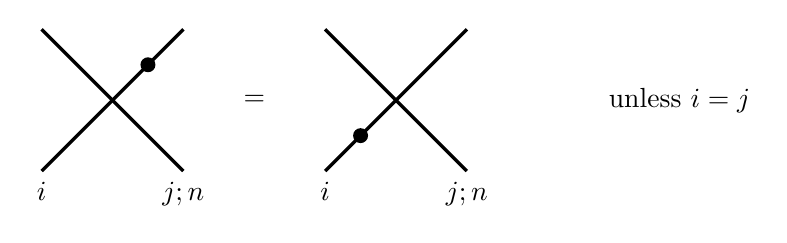
\begin{tikzpicture}[scale=.9,baseline]
      \draw[very thick](-4,0) +(-1,-1) -- +(1,1) node[below,at start]
      {$i$}; \draw[very thick](-4,0) +(1,-1) -- +(-1,1) node[below,at
      start] {$j;n$}; \fill (-3.5,.5) circle (3pt);
      % \draw[very thick] (0,0) +(0,-1) -- +(0,1) node[below, at
      % start]{$i$}; \fill (0,0) circle (5pt);
      \node at (-2,0){=}; \draw[very thick](0,0) +(-1,-1) -- +(1,1)
      node[below,at start] {$i$}; \draw[very thick](0,0) +(1,-1) --
      +(-1,1) node[below,at start] {$j;n$}; \fill (-.5,-.5) circle (3pt);
      \node at (4,0){unless $i=j$};
    \end{tikzpicture}
  \end{equation*}
  \begin{equation*}\subeqn\label{b-third-QH}
    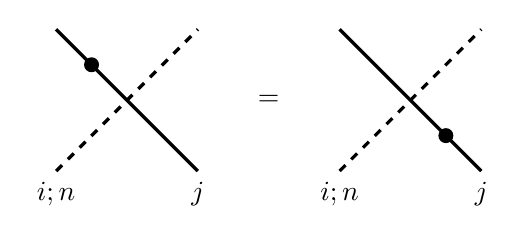
\begin{tikzpicture}[scale=.9,baseline]
      \draw[very thick,dashed](-4,0) +(-1,-1) -- +(1,1) node[below,at start]
      {$i;n$}; \draw[very thick](-4,0) +(1,-1) -- +(-1,1) node[below,at
      start] {$j$}; \fill (-4.5,.5) circle (3pt);
      % \draw[very thick] (0,0) +(0,-1) -- +(0,1) node[below, at
      % start]{$i$}; \fill (0,0) circle (5pt);
      \node at (-2,0){=}; \draw[very thick,dashed](0,0) +(-1,-1) -- +(1,1)
      node[below,at start] {$i;n$}; \draw[very thick](0,0) +(1,-1) --
      +(-1,1) node[below,at start] {$j$}; \fill (.5,-.5) circle (3pt);
    \end{tikzpicture}\qquad \qquad
    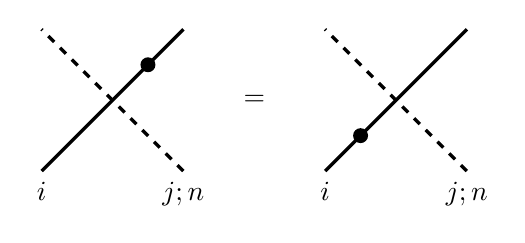
\begin{tikzpicture}[scale=.9,baseline]
      \draw[very thick](-4,0) +(-1,-1) -- +(1,1) node[below,at start]
      {$i$}; \draw[very thick,dashed](-4,0) +(1,-1) -- +(-1,1) node[below,at
      start] {$j;n$}; \fill (-3.5,.5) circle (3pt);
      % \draw[very thick] (0,0) +(0,-1) -- +(0,1) node[below, at
      % start]{$i$}; \fill (0,0) circle (5pt);
      \node at (-2,0){=}; \draw[very thick](0,0) +(-1,-1) -- +(1,1)
      node[below,at start] {$i$}; \draw[very thick,dashed](0,0) +(1,-1) --
      +(-1,1) node[below,at start] {$j;n$}; \fill (-.5,-.5) circle (3pt);
    \end{tikzpicture}
  \end{equation*}
The flavor $\phi$ acts by automorphisms of the $\gls{G}$-representation on $V$,
and thus is induced by a cocharacter into $\prod_iGL(\C^{\glslink{Bw}{w_i}})
\times\prod_{(i,j)\in {\vertex}^2} GL(\C^{\chi_{i,j}})$.  We can
assume that this cocharacter lands in the usual torus of diagonal
matrices; let $c_{i,1},\dots, c_{i,\glslink{Bw}{w_i}}$ be the weights
of its components into
$GL(\C^{\glslink{Bw}{w_i}})$ and $b_e$ for each edge $e$ the weights
of its components into $GL(\C^{\chi_{i,j}})$.
  Let
  \begin{align*}
\subeqn   \label{eq:p-def} p_{i}(u)&=\prod_{k=1}^{\glslink{Bw}{w_i}}(u-c_{i,k}-\frac{h}{2})\\
\subeqn   \label{eq:q-def} q_{ij}(u)&=\prod_{e\colon  j\to i} (u+b_e+\frac{h}{2})\cdot \prod_{e\colon
      i\to j}  (-u+b_e+\frac{h}{2}).
  \end{align*}


  This is the point where we must incorporate that our path is shifted
  by $\phi$.  Thus, when we use the relation 
  (\ref{eq:wall-cross1}) implies to switch the order of
  crossings on disjoint strands, we have:
   \begin{equation*}\subeqn\label{x-cost-1}
  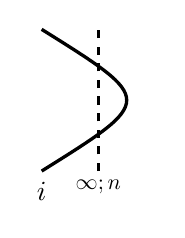
\begin{tikzpicture}[very thick,baseline,scale=.9]
    \draw (-2.8,0)  +(0,-1) .. controls (-1.2,0) ..  +(0,1) node[below,at start]{$i$};
       \draw[dashed] (-2,0)  +(0,-1)--node[below,at start,scale=.8]{$\infty;n$}  +(0,1);
  \end{tikzpicture}
=   p_{i}\Bigg(
  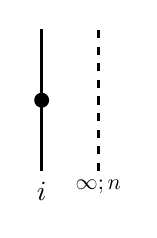
\begin{tikzpicture}[very thick,baseline,scale=.9]
 \draw[dashed] (2.3,0)  +(0,-1) -- node[below,at start,scale=.8]{$\infty;n$} +(0,1);
       \draw (1.5,0)  +(0,-1) -- +(0,1) node[below,at start]{$i$};
       \fill (1.5,0) circle (3pt);
\end{tikzpicture}-nh 
  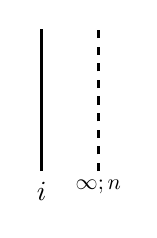
\begin{tikzpicture}[very thick,baseline,scale=.9] \draw[dashed] (2.3,0)  +(0,-1) -- node[below,at start,scale=.8]{$\infty;n$} +(0,1);
       \draw (1.5,0)  +(0,-1) -- +(0,1) node[below,at start]{$i$};
\end{tikzpicture}\Bigg)
\end{equation*}\begin{equation*}
    \subeqn\label{x-cost-2}
  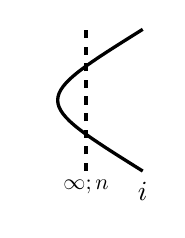
\begin{tikzpicture}[very thick,baseline,scale=.9]
          \draw[dashed] (-2,0)  +(0,-1)-- node[below,at start,scale=.8]{$\infty;n$} +(0,1);
  \draw (-1.2,0)  +(0,-1) .. controls (-2.8,0) ..  +(0,1) node[below,at start]{$i$};\end{tikzpicture}
           =p_{i}\Bigg(
  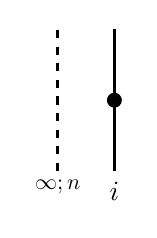
\begin{tikzpicture}[very thick,baseline,scale=.9]
    \draw (2.5,0)  +(0,-1) -- +(0,1) node[below,at start]{$i$};
       \draw[dashed] (1.7,0)  +(0,-1) -- node[below,at start,scale=.8]{$\infty;n$} +(0,1) ;
       \fill (2.5,0) circle (3pt);\end{tikzpicture}- nh  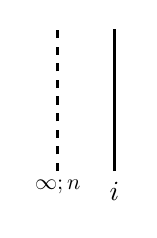
\begin{tikzpicture}[very thick,baseline,scale=.9]
    \draw (2.5,0)  +(0,-1) -- +(0,1) node[below,at start]{$i$};
       \draw[dashed] (1.7,0)  +(0,-1) -- node[below,at start,scale=.8]{$\infty;n$} +(0,1) ;
      \end{tikzpicture} \Bigg)
    \end{equation*}
   \begin{equation*}\subeqn\label{b-black-bigon1}
      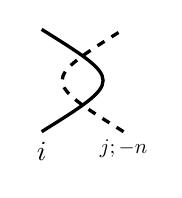
\begin{tikzpicture}[very thick,scale=.65,baseline]
      \draw(-2.8,0) +(0,-1) .. controls (-1.2,0) ..  +(0,1)
      node[below,at start]{$i$}; \draw[dashed] (-1.2,0) +(0,-1) .. controls
(-2.8,0) ..  +(0,1) node[below,at start,scale=.75]{$j;-n$};
\end{tikzpicture}\quad   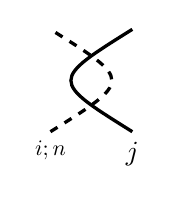
\begin{tikzpicture}[very thick,scale=.65,baseline]
      \draw[dashed] (-2.8,0) +(0,-1) .. controls (-1.2,0) ..  +(0,1)
      node[below,at start,scale=.8]{$i;n$}; \draw (-1.2,0) +(0,-1) .. controls
(-2.8,0) ..  +(0,1) node[below,at start]{$j$};
\end{tikzpicture}
=q_{ij}\Bigg(    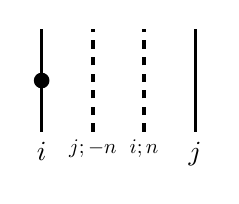
\begin{tikzpicture}[very thick,scale=.65,baseline]
      \draw(-2.8,0) +(0,-1) -- node[midway,fill=black, inner sep=2pt, circle]{} +(0,1)
      node[below,at start]{$i$}; \draw[dashed] (-1.8,0) +(0,-1) -- +(0,1) node[below,at start,scale=.75]{$j;-n$};
      \draw[dashed] (-.8,0) +(0,-1)-- +(0,1)
      node[below,at start,scale=.75]{$i;n$}; \draw (.2,0) +(0,-1) --+(0,1) node[below,at start]{$j$};
\end{tikzpicture}-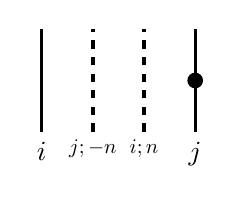
\begin{tikzpicture}[very thick,scale=.65,baseline]
      \draw(-2.8,0) +(0,-1) -- +(0,1)
      node[below,at start]{$i$}; \draw[dashed] (-1.8,0) +(0,-1) -- +(0,1) node[below,at start,scale=.75]{$j;-n$};
      \draw[dashed] (-.8,0) +(0,-1)-- +(0,1)
      node[below,at start,scale=.75]{$i;n$}; \draw (.2,0) +(0,-1) --node[midway,fill=black, inner sep=2pt, circle]{}+(0,1) node[below,at start]{$j$};
\end{tikzpicture}-nh  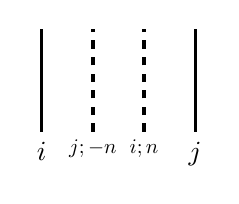
\begin{tikzpicture}[very thick,scale=.65,baseline]
      \draw(-2.8,0) +(0,-1) -- +(0,1)
      node[below,at start]{$i$}; \draw[dashed] (-1.8,0) +(0,-1) -- +(0,1) node[below,at start,scale=.75]{$j;-n$};
      \draw[dashed] (-.8,0) +(0,-1)-- +(0,1)
      node[below,at start,scale=.75]{$i;n$}; \draw (.2,0) +(0,-1) --+(0,1) node[below,at start]{$j$};
\end{tikzpicture}\Bigg)
\end{equation*}
   \begin{equation*}\subeqn\label{b-black-bigon2}
      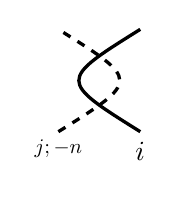
\begin{tikzpicture}[very thick,scale=.65,baseline]
      \draw (-1.2,0) +(0,-1) .. controls
(-2.8,0) ..  +(0,1) node[below,at start]{$i$};
\draw[dashed] (-2.8,0) +(0,-1) .. controls (-1.2,0) ..  +(0,1) node[below,at start,scale=.75]{$j;-n$};
\end{tikzpicture}\quad   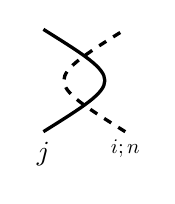
\begin{tikzpicture}[very thick,scale=.65,baseline]
      \draw[dashed] (-1.2,0) +(0,-1) .. controls
(-2.8,0) ..  +(0,1) 
      node[below,at start,scale=.75]{$i;n$}; \draw (-2.8,0) +(0,-1) .. controls (-1.2,0) ..  +(0,1) node[below,at start]{$j$};
\end{tikzpicture}
=q_{ij}\Bigg(    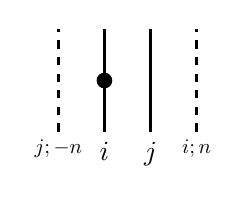
\begin{tikzpicture}[very thick,scale=.65,baseline,xscale=.9]
      \draw(-1.8,0) +(0,-1) -- node[midway,fill=black, inner sep=2pt, circle]{} +(0,1)
      node[below,at start]{$i$}; \draw[dashed] (-2.8,0) +(0,-1) -- +(0,1) node[below,at start,scale=.75]{$j;-n$};
      \draw[dashed] (.2,0) +(0,-1)-- +(0,1)
      node[below,at start,scale=.75]{$i;n$}; \draw (-.8,0) +(0,-1) --+(0,1) node[below,at start]{$j$};
\end{tikzpicture}-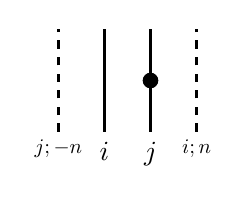
\begin{tikzpicture}[very thick,scale=.65,baseline,xscale=.9]
      \draw(-1.8,0) +(0,-1) -- +(0,1)
      node[below,at start]{$i$}; \draw[dashed] (-2.8,0) +(0,-1) -- +(0,1) node[below,at start,scale=.75]{$j;-n$};
      \draw[dashed](.2,0) +(0,-1)-- +(0,1)
      node[below,at start,scale=.75]{$i;n$}; \draw  (-.8,0)+(0,-1) --node[midway,fill=black, inner sep=2pt, circle]{}+(0,1) node[below,at start]{$j$};
\end{tikzpicture}-n h 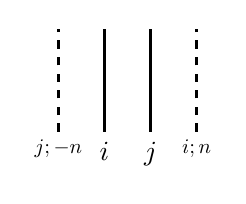
\begin{tikzpicture}[very thick,scale=.65,baseline,xscale=.9]
      \draw(-1.8,0) +(0,-1) -- +(0,1)
      node[below,at start]{$i$}; \draw[dashed] (-2.8,0) +(0,-1) -- +(0,1) node[below,at start,scale=.75]{$j;-n$};
      \draw[dashed] (.2,0) +(0,-1)-- +(0,1)
      node[below,at start,scale=.75]{$i;n$}; \draw  (-.8,0) +(0,-1) --+(0,1) node[below,at start]{$j$};
\end{tikzpicture}\Bigg)
  \end{equation*}
Note that the equations above are written assuming that $n>0$ (and
implicitly $n\in \Z-\frac{1}{2}$), but they are equally valid if $n<0$,
with the requisite reordering of strands.
The relation 
(\ref{eq:psi2}) implies that:
  \begin{equation*}\subeqn\label{b-psi2}
    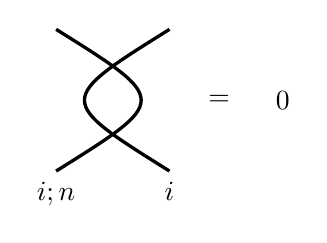
\begin{tikzpicture}[very thick,scale=.9,baseline]
      \draw (-2.8,0) +(0,-1) .. controls (-1.2,0) ..  +(0,1)
      node[below,at start]{$i;n$}; \draw (-1.2,0) +(0,-1) .. controls
      (-2.8,0) ..  +(0,1) node[below,at start]{$i$}; \node at (-.5,0)
      {=}; \node at (0.4,0) {$0$};
    \end{tikzpicture}\qquad \qquad    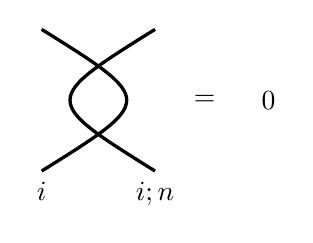
\begin{tikzpicture}[very thick,scale=.9,baseline]
      \draw (-2.8,0) +(0,-1) .. controls (-1.2,0) ..  +(0,1)
      node[below,at start]{$i$}; \draw(-1.2,0) +(0,-1) .. controls
      (-2.8,0) ..  +(0,1) node[below,at start]{$i;n$}; \node at (-.5,0)
      {=}; \node at (0.4,0) {$0$};
    \end{tikzpicture}
      \end{equation*}
The relation 
(\ref{eq:psipoly}) is equivalent to isotopy and  \begin{equation*}\subeqn\label{b-nilHecke-1}
    \begin{tikzpicture}[scale=.9,baseline]
      \draw[very thick](-4,0) +(-1,-1) -- +(1,1) node[below,at start,scale=.8]
      {$i;n$}; \draw[very thick](-4,0) +(1,-1) -- +(-1,1) node[below,at
      start] {$i$}; \fill (-4.5,.5) circle (3pt);
      % \draw[very thick] (0,0) +(0,-1) -- +(0,1) node[below, at
      % start]{$i$}; \fill (0,0) circle (5pt);
      \node at (-2,0){$-$}; \draw[very thick](0,0) +(-1,-1) -- +(1,1)
      node[below,at start,scale=.8]
      {$i;n$}; \draw[very thick](0,0) +(1,-1) --
      +(-1,1) node[below,at start] {$i$}; \fill (.5,-.5) circle (3pt);
     \node at (2,0){$=$};  \draw[very thick](4,0) +(-1,-1) -- +(-1,1)
      node[below,at start,scale=.8]
      {$i;n$}; \draw[very thick](4,0) +(0,-1) --
      +(0,1) node[below,at start] {$i$};
      \draw[weyl] (4,0) +(.5,0) -- +(-1.5,0) node[at start, right,green!50!black]{$s$} ;
    \end{tikzpicture}
  \end{equation*}
 \begin{equation*}\subeqn\label{b-nilHecke-2}
    \begin{tikzpicture}[scale=.9,baseline]
      \draw[very thick](-4,0) +(-1,-1) -- +(1,1) node[below,at
      start] {$i$}; \draw[very thick](-4,0) +(1,-1) -- +(-1,1) node[below,at start,scale=.8]
      {$i;n$}; \fill (-4.5,-.5) circle (3pt);
      % \draw[very thick] (0,0) +(0,-1) -- +(0,1) node[below, at
      % start]{$i$}; \fill (0,0) circle (5pt);
      \node at (-2,0){$-$}; \draw[very thick](0,0) +(-1,-1) -- +(1,1)
      node[below,at
      start] {$i$}; \draw[very thick](0,0) +(1,-1) --
      +(-1,1) node[below,at start,scale=.8]
      {$i;n$}; \fill (.5,.5) circle (3pt);
      \node at (2,0){$=$};  \draw[very thick](4,0) +(-1,-1) -- +(-1,1)
      node[below,at
      start] {$i$}; \draw[very thick](4,0) +(0,-1) --
      +(0,1) node[below,at start,scale=.8]
      {$i;n$}; 
      \draw[weyl] (4,0) +(.5,0) -- +(-1.5,0) node[at start, right,green!50!black]{$s$} ;
    \end{tikzpicture}
  \end{equation*}
  with $s$ denoting the unique reflection in the affine Weyl group
  switching the top and bottom labels of the diagram.

  Finally, the codimension 2 relations show how to relate the two
resolutions of a triple point. The correct relation depends on the
number of partners with the same label going through the triple
point: if all three, then we use (\ref{eq:psi}), if two we use
(\ref{eq:triple}) and if there is no such pair, then
(\ref{eq:wall-cross1}).  \excise{ Any triple point involving only partners
  \begin{equation*}\subeqn\label{b-triple-coxeter}
      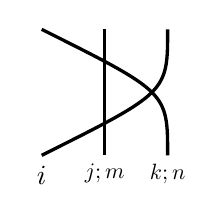
\begin{tikzpicture}[very thick,scale=.8,baseline]  \draw (1,0) +(1,-1) .. controls
      (2,0) .. +(-1,1)
      node[below,at start,scale=.8]{$k;n$}; \draw (1,0) +(-1,-1) .. controls
      (2,0) .. +(1,1)
      node[below,at start]{$i$}; \draw (1,0) +(0,-1) -- node[below, at start,scale=.8]{$j;m$}+(0,1); 
    \end{tikzpicture} =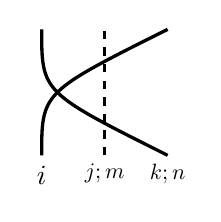
\begin{tikzpicture}[very thick,scale=.8,baseline]
      \draw (-3,0) +(1,-1) .. controls (-4,0) .. +(-1,1) node[below,at start,scale=.8]{$k;n$}; \draw
      (-3,0) +(-1,-1) .. controls (-4,0) .. +(1,1) node[below,at start]{$i$}; \draw[dashed]
      (-3,0) +(0,-1)--  node[below, at start,scale=.8]{$j;m$}+(0,1);
       \end{tikzpicture} 
  \end{equation*}
 
  Finally, the codimension 2 relation
 (\ref{eq:triple}) implies a number of different relations relating the
 two different ways of resolving a triple point
 for all 
 ghosts, we have the equation below and its reflection through a
 vertical line:
  \begin{equation*}\subeqn\label{b-triple-extra-dumb}
    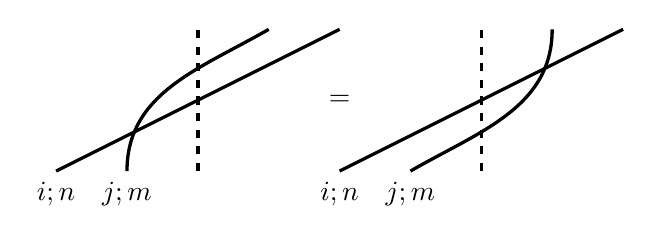
\begin{tikzpicture}[very thick,scale=.9,baseline]
      \draw (-3,0) +(-1,-1) to[out=90,in=-150] node[below,at start]{$j;m$} +(1,1) ; \draw
      (-3,0) +(-2,-1) -- +(2,1) node[below,at start]{$i;n$}; \draw[dashed]
      (-3,0) +(0,-1)--  +(0,1); \node at (-1,0) {=}; \draw (1,0) +(-1,-1) to [out=30,in=-90] node[below,at start]{$j;m$} +(1,1)
      ; \draw
      (1,0) +(-2,-1) -- +(2,1) node[below,at start]{$i;n$}; \draw[dashed] (1,0) +(0,-1) -- +(0,1); 
    \end{tikzpicture}
  \end{equation*}}
These imply we can isotope through any triple point unless it involves
exactly two partners with the label $i\in {\gls{vertex}}$.  In order to
cover this last case, let
  \begin{align*}
\partial_{m }p(u_1,u_2)&=\frac{p(u_1-mh)-p(u_2-mh)}{u_1-u_2}\\ \partial_{n,m}q(u_1,v,u_2)&=\frac{q(u_1-v+mh)-q(u_2-v+mh)}{u_1-u_2}
  \end{align*}

  \begin{equation*}\subeqn\label{b-frame-triple-smart}
      \begin{tikzpicture}[very thick,scale=.8,baseline]  \draw (1,0) +(1,-1) .. controls
      (2,0) .. +(-1,1)
      node[below,at start,scale=.8]{$i;n$}; \draw (1,0) +(-1,-1) .. controls
      (2,0) .. +(1,1)
      node[below,at start]{$i$}; \draw[dashed] (1,0) +(0,-1) -- node[above, at end,scale=.8]{$\infty;m$}+(0,1);  \draw[weyl] (1,.7) +(1.5,0) -- +(-1.5,0) node[at start, right]{$s$} ;
    \end{tikzpicture} - \begin{tikzpicture}[very thick,scale=.8,baseline]
      \draw (-3,0) +(1,-1) .. controls (-4,0) .. +(-1,1) node[below,at start,scale=.8]{$i;n$}; \draw
      (-3,0) +(-1,-1) .. controls (-4,0) .. +(1,1) node[below,at start]{$i$}; \draw[dashed]
      (-3,0) +(0,-1)--  node[above, at end,scale=.8]{$\infty;m$}+(0,1);  \draw[weyl] (-3,.7) +(1.5,0) -- +(-1.5,0) node[at start, right]{$s$} ;
       \end{tikzpicture} 
  =\partial_{n}p_i\Bigg(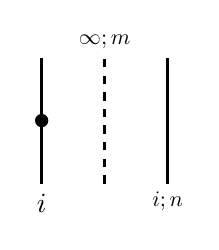
\begin{tikzpicture}[very thick,scale=.8,baseline]       \draw (0,0)
      +(1,-1) -- +(1,1) node[below,at start,scale=.8]{$i;n$};  \fill (-1,0) circle (3pt);\draw (0,0)
      +(-1,-1) -- +(-1,1) node[below,at start]{$i$}; \draw[dashed] (0,0)
      +(0,-1) -- node[above, at end,scale=.8]{$\infty;m$}+(0,1); 
    \end{tikzpicture}, 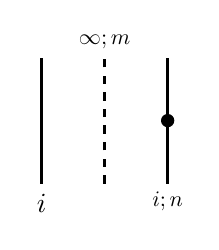
\begin{tikzpicture}[very thick,scale=.8,baseline]       \draw (0,0)
      +(1,-1) -- +(1,1) node[below,at start,scale=.8]{$i;n$};  \fill (1,0) circle (3pt);\draw (0,0)
      +(-1,-1) -- +(-1,1) node[below,at start]{$i$}; \draw[dashed] (0,0)
      +(0,-1) -- node[above, at end,scale=.8]{$\infty;m$}+(0,1);
    \end{tikzpicture}\Bigg)
  \end{equation*}
   \begin{equation*}
       \subeqn\label{b-triple-smart}
      \begin{tikzpicture}[very thick,scale=.7,baseline,xscale=.9]  \draw (1,0) +(1,-1) .. controls
      (2,0) .. +(-1,1)
      node[below,at start,scale=.8]{$i;n$}; \draw (1,0) +(-1,-1) .. controls
      (2,0) .. +(1,1)
      node[below,at start]{$i$}; \draw[dashed] (1,0) +(0,-1) -- node[above, at end,scale=.8]{$j;m$}+(0,1);  \draw[dashed] (5,0) +(1,-1) .. controls
      (6,0) .. +(-1,1)
      node[above,at end,scale=.8]{$i;\!-m$}; \draw[dashed] (5,0) +(-1,-1) .. controls
      (6,0) .. +(1,1)
      node[above,at end,scale=.8]{$i;n\!-\!m$}; \draw (5,0) +(0,-1) -- node[below, at start]{$j$}+(0,1);  \draw[weyl] (5,.4) +(1.5,0) -- +(-5.5,0) node[at start, right]{$s$} ;
    \end{tikzpicture}  
    %\begin{tikzpicture}[very thick,scale=.7,baseline,xscale=.9]  \draw (1,0) +(1,-1) .. controls
    %  (2,0) .. +(-1,1)
    %  node[below,at start]{$i$}; \draw (1,0) +(-1,-1) .. controls
    %  (2,0) .. +(1,1)
    %  node[below,at start,scale=.8]{$i;\!-n$}; \draw[dashed] (1,0) +(0,-1) -- node[above, at end,scale=.8]{$j;m\!-\!n$}+(0,1); 
    %\end{tikzpicture}   
    - \begin{tikzpicture}[very thick,scale=.7,baseline,xscale=.9]
      \draw (-3,0) +(1,-1) .. controls (-4,0) .. +(-1,1) node[below,at start,scale=.8]{$i;n$}; \draw
      (-3,0) +(-1,-1) .. controls (-4,0) .. +(1,1) node[below,at start]{$i$}; \draw[dashed]
      (-3,0) +(0,-1)--  node[above, at end,scale=.8]{$j;m$}+(0,1);  
      \draw[dashed] (1,0) +(1,-1) .. controls (0,0) .. +(-1,1) node[above,at end,scale=.8]{$i;\!-m$}; \draw[dashed]
      (1,0) +(-1,-1) .. controls (0,0) .. +(1,1) node[above,at end,scale=.8]{$i;n\!-\!m$}; \draw
      (1,0) +(0,-1)--  node[below, at start]{$j$}+(0,1);  \draw[weyl] (-1,.4) +(3.5,0) -- +(-3.5,0) node[at start, right]{$s$} ;
       \end{tikzpicture} 
       %\begin{tikzpicture}[very thick,scale=.7,baseline,xscale=.9]
      %\draw (-3,0) +(1,-1) .. controls (-4,0) .. +(-1,1) %node[below,at start,scale=.8]{$i;n$}; \draw
      %(-3,0) +(-1,-1) .. controls (-4,0) .. +(1,1) node[below,at %start,scale=.8]{$i;\!-n$}; \draw[dashed]
      %(-3,0) +(0,-1)--  node[above, at %end,scale=.8]{$j;m\!-\!n$}+(0,1);
       %\end{tikzpicture} 
  =\partial_{n,m}q_{ij}(\gamma_1, \gamma_2, \gamma_3)
\end{equation*}
\begin{equation*}
 \gamma_1=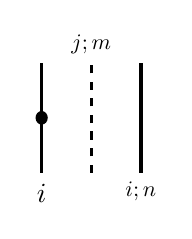
\begin{tikzpicture}[very thick,scale=.7,baseline,xscale=.9]       \draw (0,0)
      +(1,-1) -- +(1,1) node[below,at start,scale=.8]{$i;n$};  \fill (-1,0) circle (3.5pt);\draw (0,0)
      +(-1,-1) -- +(-1,1) node[below,at start]{$i$}; \draw[dashed] (0,0)
      +(0,-1) -- node[above, at end,scale=.8]{$j;m$}+(0,1); 
    \end{tikzpicture} 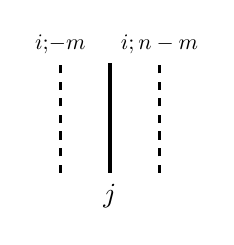
\begin{tikzpicture}[very
      thick,scale=.7,baseline,xscale=.9]  \draw[dashed] (1,0) +(1,-1) -- +(1,1)
      node[above,at end,scale=.8]{$i;n-m$}; \draw[dashed] (1,0) +(-1,-1) --+(-1,1)
      node[above,at end,scale=.8]{$i;\!-m$}; \draw (1,0) +(0,-1) -- node[below, at start]{$j$}+(0,1); 
    \end{tikzpicture}
    %\begin{tikzpicture}[very thick,scale=.7,baseline,xscale=.9]    %   \draw (0,0)
    %  +(1,-1) -- +(1,1) node[below,at start]{$i$}; \draw (0,0)
%      +(-1,-1) -- +(-1,1) node[below,at start,scale=.8]{$i;\!-n$}; \draw[dashed] (0,0)
 %     +(0,-1) -- node[above, at end,scale=.8]{$j;m\!-\!n$}+(0,1); 
    %\end{tikzpicture}  
    \quad  \gamma_2= \begin{tikzpicture}[very thick,scale=.7,baseline,xscale=.9]       \draw (0,0)
      +(1,-1) -- +(1,1) node[below,at start,scale=.8]{$i;n$};  \draw (0,0)
      +(-1,-1) -- +(-1,1) node[below,at start]{$i$}; \draw[dashed] (0,0)
      +(0,-1) -- node[above, at end,scale=.8]{$j;m$}+(0,1); 
    \end{tikzpicture}\begin{tikzpicture}[very
      thick,scale=.7,baseline,xscale=.9]  \draw[dashed] (1,0) +(1,-1) -- +(1,1)
      node[above,at end,scale=.8]{$i;n-m$}; \draw[dashed] (1,0) +(-1,-1) --+(-1,1)
      node[above,at end,scale=.8]{$i;\!-m$}; \draw (1,0) +(0,-1) -- node[below, at start]{$j$}+(0,1); \fill (1,0) circle (3.5pt);
    \end{tikzpicture}
   % \begin{tikzpicture}[very thick,scale=.7,baseline,xscale=.9]     %  \draw (0,0)
    %  +(1,-1) -- +(1,1) node[below,at start]{$i$}; \draw (0,0)
    %  +(-1,-1) -- +(-1,1) node[below,at start,scale=.8]{$i;\!-n$}; %\draw[dashed] (0,0)
    %  +(0,-1) -- node[above, at end,scale=.8]{$j;m\!-\!n$}+(0,1); 
%    \end{tikzpicture} 
  %  \end{equation*}
%\begin{equation*} 
\quad
\gamma_3= \begin{tikzpicture}[very thick,scale=.7,baseline,xscale=.9]       \draw (0,0)
      +(1,-1) -- +(1,1) node[below,at start,scale=.8]{$i;n$};  \draw (0,0)
      +(-1,-1) -- +(-1,1) node[below,at start]{$i$}; \draw[dashed] (0,0)
      +(0,-1) -- node[above, at end,scale=.8]{$j;m$}+(0,1);       \fill (1,0) circle (3.5pt);
    \end{tikzpicture}\begin{tikzpicture}[very
      thick,scale=.7,baseline,xscale=.9]  \draw[dashed] (1,0) +(1,-1) -- +(1,1)
      node[above,at end,scale=.8]{$i;n-m$}; \draw[dashed] (1,0) +(-1,-1) --+(-1,1)
      node[above,at end,scale=.8]{$i;\!-m$}; \draw (1,0) +(0,-1) -- node[below, at start]{$j$}+(0,1); 
    \end{tikzpicture}
    %\begin{tikzpicture}[very thick,scale=.7,baseline,xscale=.9]       \draw (0,0)
    %  +(1,-1) -- +(1,1) node[below,at start]{$i$}; \draw (0,0)
    %  +(-1,-1) -- +(-1,1) node[below,at start,scale=.8]{$i;\!-n$}; %\draw[dashed] (0,0)
    %  +(0,-1) -- node[above, at end,scale=.8]{$j;m\!-\!n$}+(0,1); 
%    \end{tikzpicture} 
  \end{equation*}
  with $s$ denoting the unique reflection in the affine Weyl group
  making the top and bottom match.  As before, using $p$ and $q$
  accounts for our shift by $\gls{flav}$.

  Given this reinterpretation of our relations in terms of diagrams, this allows us to interpret the relations (\ref{eq:dot-migration}--\ref{b-triple-smart}) as relations on unrolled diagrams, by setting $\sum a_iD_i=0$ if we have that $\sum a_i\mathbbm{r}_{D_i}=0$.
  In this case, we have that:
  \begin{lemma}\label{lem:unrolled-B}
    Given $\eta,\eta'\in \ft_{\second}$, the Hom space
    $\Hom_{\gls{scrB}}(\eta,\eta')$ is spanned by the morphisms
    $\mathbbm{r}_D$ for unrolled diagrams $D$ with top $\eta'$ and
    bottom $\eta$, modulo the local relations (\ref{eq:dot-migration}--\ref{b-triple-smart}).
  \end{lemma}
  \begin{proof}
    We have justified in each individual case why the relations
    (\ref{eq:dot-migration}--\ref{b-triple-smart}) hold.  Thus, we have a
    map from the formal span of unrolled diagrams modulo these
    relations to $\Hom_{\mathscr{B}}(\eta,\eta')$.  This is surjective
    because the generating morphisms of the category $\mathscr{B}$ are
    given by the basic unrolled diagrams in
    \eqref{eq:unrolled-possible}.  On the other hand, the relations
    (\ref{eq:dot-migration}--\ref{b-triple-smart}) suffice to write any
     $\mathbbm{r}_D$ as a sum of diagrams corresponding to a reduced word in
    $\widehat{W}$ with all dots and green lines at the bottom, and to
    relate any two reduced words for $w\in \widehat{W}$ modulo the
    diagrams for shorter elements of $\widehat{W}$.  Thus, we find
    that the unrolled diagrams corresponding to the basis of
    \cite[Cor. 3.12]{WebSD} are a spanning set of this quotient.  This
    is only possible if the map is injective as well.
  \end{proof}
  
\subsection{Antipodal diagrams}
\label{sec:antipodal-diagrams}

  The reader may have noticed that these diagrams are actually quite
  difficult to draw and interpret, but there is a symmetry that we
  have not exploited, the action of the extended affine Weyl group.
  The quotient of $\prod_i\R^{\glslink{Bv}{v_i}}$ by the extended Weyl group is
  given by the space $\prod_i (\R/\Z)^{v_i}/S_{v_i}$, which we can
  interpret as the moduli space of multisubsets of the circle $\R/\Z$
  labeled with elements of ${\gls{vertex}}$, such that $v_i$ elements have label $i\in {\vertex}$.
  Thus the path $[0,1]\to \prod_i\R^{v_i}$ composed
  with the projection $\prod_i\R^{v_i}\to \prod_i
  (\R/\Z)^{v_i}/S_{v_i}$ can be thought of as a path in 
  this moduli space.

  We draw this by considering our diagrams in $\R\times [0,1]$, and
  considering the quotient of this plane by $\Z$ acting by addition to
  the $x$-coordinate.  Note that this sends all the partners to
  a single curve in  $\R/\Z\times [0,1]$, and all  ghosts
  to a single curve $\frac{1}{2}$ units in either direction (since we
  are on a circle).  We can describe the
  resulting diagrams as follows:

 \begin{definition}\label{def:cyl-BFN}
  An {\bf antipodal diagram} is a collection of finitely many
  oriented curves in $\R/\Z\times [0,1]$ of the form
  $\{(\bar{\pi}(t),t)\mid t\in [0,1]\}$ for some path $\bar{\pi}\colon
  [0,1]\to \R/\Z$.
  Each curve is labeled with an element $i\in {\gls{vertex}}$ and decorated with
  finitely many dots.  For each curve, we draw a ``ghost'' curve at
  $\{(\bar{\pi}(t)-\frac{1}{2},t)\mid t\in [0,1]\}$, as well as one at
  $\{(-\frac{1}{2},t)\mid t\in [0,1]\}$. 
  We draw these as dashed.

  The diagram must be locally of the
  form given in \eqref{eq:unrolled-possible}.
That is, there are no tangencies, triple crossings or dots on
crossings.  The curves (including ghosts) must
meet the circles at
$y=0$ and $y=1$ at distinct points. We consider these
diagrams 
up to isotopy preserving the conditions above.  
\end{definition}

We call a subset of $\R/\Z$ {\bf generic} if the distance between no pair of elements is $\frac{1}{2}$.  Our conditions above guarantee that for a fixed $t$, the elements $\bar{\pi}(t)$ for the different strands are distinct and form a generic subset if and only if no pair of strands or strand and ghost cross at height $t$.

Every antipodal diagram has a unique lift to a path $[0,1]\to \ft_{\tau}$ which starts in the fundamental region of $\widehat{W}$ where the coordinates $z_{i,k}$ satisfy
\begin{equation}
    -\frac{1}{2}< z_{i,1}<z_{i,2}<\cdots < z_{i,\glslink{Bv}{v_i}}<\frac{1}{2}.  
\end{equation}
That is, by the path lifting property of the universal cover, each of the curves $\bar{\pi}\colon [0,1]\to \R/\Z$ has a unique lift $\pi$ with $-\frac{1}{2}<\pi(0)<\frac{1}{2}$, and we can number these so that \begin{equation}
    -\frac{1}{2}<\pi_{i,1}(0)<\cdots <\pi_{i,v_i}(0)<\frac{1}{2}.
\end{equation} 
\begin{definition}\label{def:antipodal-r}
 Given an antipodal diagram $D$ with no dots, let $\mathbbm{r}_D$ be the morphism defined by the lifted path starting in the fundamental region, followed by the unique element of $\widehat{W}$ sending us back to the fundamental region.    
 
 If the diagram does contain dots, then place these in the lifted diagram on the unique partner preimage which has $x$-value in $(-\frac{1}{2}, \frac{1}{2} )$.
\end{definition}
We have to be careful about lifting antipodal diagrams with dots,
because if we do so in the most naive way, the result will not be
compatible with composition, which the definition above is.  We could accomplish the same effect if instead of 
applying a Weyl group element at the end, we  applied one
immediately whenever we left the fundamental region to move back into
it.  

We can also modify the relations
(\ref{eq:dot-migration}--\ref{b-triple-smart}) to work as relations on
antipodal diagrams, as before following the rule that $\sum a_iD_i=0$
if we have that $\sum a_i\mathbbm{r}_{D_i}=0$.  Some of these can
interpreted locally exactly as they read above:
(\ref{b-first-QH}--\ref{b-second-QH}) and
(\ref{b-psi2}--\ref{b-nilHecke-2}) are of this type. On the other, if
a dot on an antipodal diagram is slid over the half-integer ghost with
label $\infty$, then it goes between lifting to the ghost just right
of $x=-\frac{1}{2}$ to that just left of $x=\frac{1}{2}$.  The effect
of (\ref{eq:dot-migration})  is thus the following relation on antipodal diagrams: \newseq
    \begin{equation*}\subeqn\label{a-dot-slide}
    \begin{tikzpicture}[very thick,baseline,scale=.7]
  \draw(-3,0) +(-1,-1) -- +(1,1);
  \draw[dashed](-3,0) +(0,-1) -- node[below,at start]{$\infty$}  +(0,1);
\fill (-3.5,-.5) circle (3pt); \end{tikzpicture}
=
 \begin{tikzpicture}[very thick,baseline,scale=.7] \draw(1,0) +(-1,-1) -- +(1,1);
  \draw[dashed](1,0) +(0,-1) -- node[below,at start]{$\infty$}  +(0,1);
\fill (1.5,.5) circle (3pt);
    \end{tikzpicture} +h  \begin{tikzpicture}[very thick,baseline,scale=.7] \draw(1,0) +(-1,-1) -- +(1,1);
  \draw[dashed](1,0) +(0,-1) -- node[below,at start]{$\infty$}  +(0,1);
    \end{tikzpicture}
\qquad \qquad     \begin{tikzpicture}[very thick,baseline,scale=.7]
  \draw(-3,0) +(1,-1) -- +(-1,1);
  \draw[dashed](-3,0) +(0,-1) -- node[below,at start]{$\infty$}  +(0,1);
\fill (-2.5,-.5) circle (3pt); \end{tikzpicture}
=
 \begin{tikzpicture}[very thick,baseline,scale=.7] \draw(1,0) +(1,-1) -- +(-1,1);
  \draw[dashed](1,0) +(0,-1) -- node[below,at start]{$\infty$}  +(0,1);
\fill (.5,.5) circle (3pt);
    \end{tikzpicture} -h  \begin{tikzpicture}[very thick,baseline,scale=.7] \draw(1,0) +(1,-1) -- +(-1,1);
  \draw[dashed](1,0) +(0,-1) --node[below,at start]{$\infty$}   +(0,1);
    \end{tikzpicture}
  \end{equation*}
The other relations need to interpreted carefully to be compatible with lifting. For example, the relations (\ref{x-cost-1}--\ref{x-cost-2}) become
  \begin{equation*}\subeqn\label{a-cost-1}
  \begin{tikzpicture}[very thick,baseline,scale=.9]
    \draw (-2.8,0)  +(0,-1) .. controls (-1.2,0) ..  +(0,1) node[below,at start]{$i$};
       \draw[dashed] (-2,0)  +(0,-1)--node[below,at start]{$\infty$}  +(0,1);
  \end{tikzpicture}
=   p_{i}\Bigg(
  \begin{tikzpicture}[very thick,baseline,scale=.9]
 \draw[dashed] (2.3,0)  +(0,-1) -- node[below,at start]{$\infty$} +(0,1);
       \draw (1.5,0)  +(0,-1) -- +(0,1) node[below,at start]{$i$};
       \fill (1.5,0) circle (3pt);
\end{tikzpicture}-\frac{1}{2}h 
  \begin{tikzpicture}[very thick,baseline,scale=.9] \draw[dashed] (2.3,0)  +(0,-1) -- node[below,at start]{$\infty$} +(0,1);
       \draw (1.5,0)  +(0,-1) -- +(0,1) node[below,at start]{$i$};
\end{tikzpicture}\Bigg)
\end{equation*}\begin{equation*}
    \subeqn\label{a-cost-2}
  \begin{tikzpicture}[very thick,baseline,scale=.9]
          \draw[dashed] (-2,0)  +(0,-1)-- node[below,at start]{$\infty$} +(0,1);
  \draw (-1.2,0)  +(0,-1) .. controls (-2.8,0) ..  +(0,1) node[below,at start]{$i$};\end{tikzpicture}
           =p_{i}\Bigg(
  \begin{tikzpicture}[very thick,baseline,scale=.9]
    \draw (2.5,0)  +(0,-1) -- +(0,1) node[below,at start]{$i$};
       \draw[dashed] (1.7,0)  +(0,-1) -- node[below,at start]{$\infty$} +(0,1) ;
       \fill (2.5,0) circle (3pt);\end{tikzpicture}+ \frac{1}{2}h  \begin{tikzpicture}[very thick,baseline,scale=.9]
    \draw (2.5,0)  +(0,-1) -- +(0,1) node[below,at start]{$i$};
       \draw[dashed] (1.7,0)  +(0,-1) -- node[below,at start]{$\infty$} +(0,1) ;
      \end{tikzpicture} \Bigg)
    \end{equation*}
Similarly, the relations (\ref{b-black-bigon1}--\ref{b-black-bigon1}) depend on the cyclic order of the strands $i,j$ and the point $x=-\frac{1}{2}$ on the circle.  Assuming these are cyclically ordered, we have:
  \begin{equation*}\subeqn\label{a-black-bigon1}
      \begin{tikzpicture}[very thick,scale=.65,baseline]
      \draw(-2.8,0) +(0,-1) .. controls (-1.2,0) ..  +(0,1)
      node[below,at start]{$i$}; \draw[dashed] (-1.2,0) +(0,-1) .. controls
(-2.8,0) ..  +(0,1) node[below,at start]{$j$};
\end{tikzpicture}\quad   \begin{tikzpicture}[very thick,scale=.65,baseline]
      \draw[dashed] (-2.8,0) +(0,-1) .. controls (-1.2,0) ..  +(0,1)
      node[below,at start]{$i$}; \draw (-1.2,0) +(0,-1) .. controls
(-2.8,0) ..  +(0,1) node[below,at start]{$j$};
\end{tikzpicture}
=q_{ij}\Bigg(    \begin{tikzpicture}[very thick,scale=.65,baseline]
      \draw(-2.8,0) +(0,-1) -- node[midway,fill=black, inner sep=2pt, circle]{} +(0,1)
      node[below,at start]{$i$}; \draw[dashed] (-1.8,0) +(0,-1) -- +(0,1) node[below,at start]{$j$};
      \draw[dashed] (-.8,0) +(0,-1)-- +(0,1)
      node[below,at start]{$i$}; \draw (.2,0) +(0,-1) --+(0,1) node[below,at start]{$j$};
\end{tikzpicture}-\begin{tikzpicture}[very thick,scale=.65,baseline]
      \draw(-2.8,0) +(0,-1) -- +(0,1)
      node[below,at start]{$i$}; \draw[dashed] (-1.8,0) +(0,-1) -- +(0,1) node[below,at start]{$j$};
      \draw[dashed] (-.8,0) +(0,-1)-- +(0,1)
      node[below,at start]{$i$}; \draw (.2,0) +(0,-1) --node[midway,fill=black, inner sep=2pt, circle]{}+(0,1) node[below,at start]{$j$};
\end{tikzpicture}-\frac{1}{2}h  \begin{tikzpicture}[very thick,scale=.65,baseline]
      \draw(-2.8,0) +(0,-1) -- +(0,1)
      node[below,at start]{$i$}; \draw[dashed] (-1.8,0) +(0,-1) -- +(0,1) node[below,at start]{$j$};
      \draw[dashed] (-.8,0) +(0,-1)-- +(0,1)
      node[below,at start]{$i$}; \draw (.2,0) +(0,-1) --+(0,1) node[below,at start]{$j$};
\end{tikzpicture}\Bigg)
\end{equation*}
   \begin{equation*}\subeqn\label{a-black-bigon2}
      \begin{tikzpicture}[very thick,scale=.65,baseline]
      \draw (-1.2,0) +(0,-1) .. controls
(-2.8,0) ..  +(0,1) node[below,at start]{$i$};
\draw[dashed] (-2.8,0) +(0,-1) .. controls (-1.2,0) ..  +(0,1) node[below,at start]{$j$};
\end{tikzpicture}\quad   \begin{tikzpicture}[very thick,scale=.65,baseline]
      \draw[dashed] (-1.2,0) +(0,-1) .. controls
(-2.8,0) ..  +(0,1) 
      node[below,at start]{$i$}; \draw (-2.8,0) +(0,-1) .. controls (-1.2,0) ..  +(0,1) node[below,at start]{$j$};
\end{tikzpicture}
=q_{ij}\Bigg(    \begin{tikzpicture}[very thick,scale=.65,baseline,xscale=.9]
      \draw(-1.8,0) +(0,-1) -- node[midway,fill=black, inner sep=2pt, circle]{} +(0,1)
      node[below,at start]{$i$}; \draw[dashed] (-2.8,0) +(0,-1) -- +(0,1) node[below,at start]{$j$};
      \draw[dashed] (.2,0) +(0,-1)-- +(0,1)
      node[below,at start]{$i$}; \draw (-.8,0) +(0,-1) --+(0,1) node[below,at start]{$j$};
\end{tikzpicture}-\begin{tikzpicture}[very thick,scale=.65,baseline,xscale=.9]
      \draw(-1.8,0) +(0,-1) -- +(0,1)
      node[below,at start]{$i$}; \draw[dashed] (-2.8,0) +(0,-1) -- +(0,1) node[below,at start]{$j$};
      \draw[dashed](.2,0) +(0,-1)-- +(0,1)
      node[below,at start]{$i$}; \draw  (-.8,0)+(0,-1) --node[midway,fill=black, inner sep=2pt, circle]{}+(0,1) node[below,at start]{$j$};
\end{tikzpicture}-\frac{1}{2} h \begin{tikzpicture}[very thick,scale=.65,baseline,xscale=.9]
      \draw(-1.8,0) +(0,-1) -- +(0,1)
      node[below,at start]{$i$}; \draw[dashed] (-2.8,0) +(0,-1) -- +(0,1) node[below,at start]{$j$};
      \draw[dashed] (.2,0) +(0,-1)-- +(0,1)
      node[below,at start]{$i$}; \draw  (-.8,0) +(0,-1) --+(0,1) node[below,at start]{$j$};
\end{tikzpicture}\Bigg)
  \end{equation*}
Since we can switch $i$ and $j$ without loss of generality, we do not need a second version of these relations.  
\begin{definition}  The {\bf antipodal KLR category}  is the category whose \begin{itemize}
    \item objects are generic subsets  of $\R/\Z$, labeled with elements of ${\gls{vertex}}$, with $\glslink{Bv}{v_i}$ having label $i$.
    \item morphisms are the quotient of the formal span of antipodal diagrams
  over $\K[c_{*,*},b_*]$  modulo the relations induced by (\ref{eq:dot-migration}--\ref{b-triple-smart}), in particular  by (\ref{a-dot-slide}--\ref{a-black-bigon2}).  
\end{itemize}  
% We let the {\bf cylindrical BFN category} be the category whose objects are subsets of $(\R/\Z)\setminus \{0\}$, with each element of the subset labeled with $i\in \gls{quiver}$, and whose morphisms are cylindrical KLR diagrams with the source at bottom and target at top.  
\end{definition}
Some might prefer to think about the antipodal KLR algebra, which is
the endomorphisms of the formal sum of all objects in this category.
Lemma \ref{lem:unrolled-B} can thus be rephrased as:
\begin{proposition}\label{prop:KLR-B}
The antipodal KLR category is equivalent to the category $\gls{scrB}$. 
\end{proposition}
Note, this construction is closely related to the flag Yangian introduced in \cite[Def. 4.12]{KTWWY2}.  In that paper, we assumed that $\gls{quiver} $ was bipartite (with the sets of nodes called {\bf even} and {\bf odd}), 
that if $i\to j$ then $i$ is even and $j$ odd.  Furthermore, the
definition depended on a polynomial $p_i$.  If 
$h=2$, $b_e=0$ and the scalars $c_{i,k}$ are the roots (with
multiplicity) of $p_i(2u-1)$, then the antipodal KLR category is
closely related to the flag Yangian category,
via the transformation  of diagrams sending all odd strands to their
antipodal ghosts.  Since there are some minor differences between
these categories, we will not make a precise statement about the
relationship between them.  


Let us give a simple example. Consider  $\gls{G}=GL(2)$ and $\gls{V}\cong \C^2\oplus \mathfrak{gl}_2$.  We have a natural isomorphism $\ft_{\R}\cong \R^2$ with the coordinates given by $z_{1},z_{2}$.  The unrolled matter hyperplanes are $z_1,z_2,z_1-z_2\in \Z-\frac{1}{2}$ and the unrolled root hyperplanes are $\alpha= z_1-z_2\in \Z$.  

With these conventions, we match morphisms of the extended category with antipodal diagrams.  We'll draw these on a cylinder sliced open at $x=\frac{1}{2}$.  
\begin{equation*} 
       \tikz[very thick,scale=.8,baseline]{
\draw (1.2,2.5)-- (1.2,-2.5) node[at start,above,scale=.8]{$z_1=\frac{1}{2}$}; \draw (-1.2,2.5)--
(-1.2,-2.5) node[at start,above,scale=.8]{$z_1=-\frac{1}{2}$};
\draw (2.5,1.2)-- (-2.5,1.2) node[at start,right,scale=.8]{$z_2=\frac{1}{2}$}; \draw (2.5,-1.2)--
(-2.5,-1.2) node[at start,right,scale=.8]{$z_2=-\frac{1}{2}$}; 
 \draw[dotted] (-2.5,-2.5) -- node[above right,at
        end,scale=.8]{$\alpha=0$}(2.5,2.5); 
        \draw(-2.5,-1.3) -- node[left,at
        start,scale=.8]{$\alpha=\frac{1}{2}$}(1.3,2.5); 
         \draw (-1.3,-2.5) -- node[left,at
        start,scale=.8]{$\alpha=-\frac{1}{2}$}(2.5,1.3); 
 \draw[dotted] (-2.5,-.1) -- node[left ,at
        start,scale=.8]{$\alpha=-1$}(.1,2.5); 
 \draw[dotted] (-.1,-2.5) -- node[right,at
        end,scale=.8]{$\alpha=1$}(2.5,.1); 
\draw[->,dashed] (-.8,.8) to (.3,-.3);
}\qquad \leftrightarrow \qquad
       \tikz[very thick,xscale=1.5,baseline]{
          \draw[fringe] (-1,-1)-- (-1,1);
          \draw[fringe] (1,1)-- (1,-1);
           \draw (.8 ,-1) to (-.3,1);
        \draw (-.8 ,-1) to (.3,1);
        \draw[dashed] (-.2,-1) -- (-1,0.45454545454);
        \draw[dashed] (.2,-1) -- (1,0.45454545454);
        \draw[dashed] (-.7,1) -- (-1,0.45454545454);
        \draw[dashed] (.7,1) -- (1,0.45454545454);
        }
\end{equation*}
\begin{equation*} 
       \tikz[very thick,scale=.8,baseline]{
\draw (1.2,2.5)-- (1.2,-2.5) node[at start,above,scale=.8]{$z_1=\frac{1}{2}$}; \draw (-1.2,2.5)--
(-1.2,-2.5) node[at start,above,scale=.8]{$z_1=-\frac{1}{2}$};
\draw (2.5,1.2)-- (-2.5,1.2) node[at start,right,scale=.8]{$z_2=\frac{1}{2}$}; \draw (2.5,-1.2)--
(-2.5,-1.2) node[at start,right,scale=.8]{$z_2=-\frac{1}{2}$}; 
 \draw[dotted] (-2.5,-2.5) -- node[above right,at
        end,scale=.8]{$\alpha=0$}(2.5,2.5); 
                \draw (-2.5,-1.3) -- node[left,at
        start,scale=.8]{$\alpha=\frac{1}{2}$}(1.3,2.5); 
         \draw (-1.3,-2.5) -- node[left,at
        start,scale=.8]{$\alpha=-\frac{1}{2}$}(2.5,1.3); 
 \draw[dotted] (-2.5,-.1) -- node[left ,at
        start,scale=.8]{$\alpha=-1$}(.1,2.5); 
 \draw[dotted] (-.1,-2.5) -- node[right,at
        end,scale=.8]{$\alpha=1$}(2.5,.1); 
\draw[->,dashed] (-.7,0) to (-.1,1.8);
}\qquad \leftrightarrow \qquad
       \tikz[very thick,xscale=1.5,baseline]{
          \draw[fringe] (-1,-1)-- (-1,1);
          \draw[fringe] (1,1)-- (1,-1);
           \draw[dashed] (-1 ,-1) to(.8,1);
        \draw (-.7 ,-1) to (-.1,1);
        \draw[dashed] (.3 ,-1) to (.9,1);     
        \draw (0 ,-1) to (1,0.1111111111);
            \draw (-1 ,0.1111111111) to (-.2,1);
        \draw[dashed] (.3 ,-1) to (.9,1); }
\end{equation*}


\subsection{Representations}

We can also naturally study the weight modules over the extended category in
this framework.  

By Proposition \ref{prop:B-equiv} and Theorem \ref{thm:pStein-equiv}, we can use this description to understand the category of $\EuScript{A}$-modules.  
We will assume again for simplicity that $\K=\mathbb{F}_p$.  Thus, all roots and weights are relevant.  

Now, we consider how our diagrams change under taking \gls{pthroot} conventions (as in Definition \ref{def:pth-root}). The structure of our diagrams will depend on the flavor parameters $b_e,c_{i,k}\in \Z.$  In particular, in our usual parameters, 
the unrolled root hyperplanes are unchanged and thus are the same as \eqref{eq:unroll-root} and the unrolled
matter hyperplanes become:
\begin{align*}\subeqn\label{eq:unroll-matter3}
z_{j,k}-z_{i,m}&=n-\frac{b_e}{p}-\frac{1}{2p}\qquad \text{ for all edges } e\colon i\to j,
  k\in [1,\glslink{Bv}{v_j}], m\in [1,\glslink{Bv}{v_i}], n\in \Z\\
\subeqn z_{i,m}&=n-\frac{c_{i,k}}{p}-\frac{1}{2p}\qquad \text{ for all } i\in {\vertex}, m\in [1,\glslink{Bv}{v_i}], k\in [1,\glslink{Bw}{w_i}], n\in \Z\label{eq:unroll-matter4}
\end{align*}


\begin{definition}
 A {\bf weighted antipodal} diagram is a collection 
 of finitely many
  oriented curves in $\R/\Z\times [0,1]$ of the form
  $\{(\bar{\pi}(t),t)\mid t\in [0,1]\}$ for some path $\bar{\pi}\colon
  [0,1]\to \R/\Z$.
  Just as before, each curve is labeled with an element $i\in {\gls{vertex}}$ and decorated with
  finitely many dots.  For each curve with label $i$, and each edge $i\to j$, we draw a ``ghost'' curve at
  $\{(\bar{\pi}(t)-\frac{b_e}{p}-\frac{1}{2p},t)\mid t\in [0,1]\}$, which we
  draw as dashed. We also draw the ghosts of infinity at
  $x=-\frac{c_{i,k}}{p}-\frac{1}{2p}$ as red.  These should satisfy the 
  same genericity conditions as antipodal diagrams, in particular, the
  local possibilities all appear below:
  \begin{equation*}
    \begin{tikzpicture}[scale=.8]
        \draw[very thick] (-12,0) +(-1,-1) -- +(1,1);
 
  \draw[very thick, dashed](-12,0) +(1,-1) -- +(-1,1);
 


  \draw[very thick, dashed] (-8,0) +(-1,-1) -- +(1,1);
 
  \draw[very thick](-8,0) +(1,-1) -- +(-1,1);
  \draw[very thick] (-4,0) +(-1,-1) -- +(1,1);
   % node[below,at start] {$i$};
  \draw[very thick](-4,0) +(1,-1) -- +(-1,1);
  %  node[below,at start] {$j$};

%\draw[very thick] (0,0) +(0,-1) -- +(0,1)
%node[below, at start]{$i$};
%\fill (0,0) circle (5pt);


  \draw[very thick](-1,0) +(0,-1) --  node
  [midway,circle,fill=black,inner sep=2pt]{}
  +(0,1);
  
  \draw[very thick] (2,0) +(-1,-1) -- +(1,1);
   % node[below,at start] {$i$};
  \draw[very thick,wei](2,0) +(0,-1) -- +(0,1);
  
  \draw[very thick] (5,0) +(1,-1) -- +(-1,1);
   % node[below,at start] {$i$};
  \draw[very thick,wei](5,0) +(0,-1) -- +(0,1);
\end{tikzpicture}
\end{equation*}

As in \cite{WebwKLR}, we let a {\bf cylindrical loading} be a map to ${\gls{vertex}}$ from
a finite subset of $\R/\Z$ which avoids
    $x=-\frac{c_{i,k}}{p}-\frac{1}{2p}$ and such that if there is an edge
    $e\colon i\to j$, then there is no pair of
    elements $x$ and $y$ mapping to $i$ and $j$ with
    $x-y=\frac{b_e}{p}+\frac{1}{2p}$. Note that  the top and bottom of each weighted
    antipodal diagram gives a cylindrical loading.
\end{definition}
Note the similarity of these diagrams to {\bf weighted KLR diagrams}
as defined in \cite{WebwKLR}.  Just as antipodal diagrams define morphisms in \gls{scrB}, weighted antipodal diagrams define morphisms in \gls{sfB}.  The relations of $\gls{sfB}$ thus induce an appropriate
modification of the relations
(\ref{eq:dot-migration}--\ref{b-triple-smart}), where we set $h=0$ (which
greatly simplifies them) and change of flavor means that we separate the contributions in
(\ref{a-cost-1}--\ref{a-black-bigon2}) into the different ghost
strands.  That is, assuming that all $b_e$ and $c_{i,k}$'s are different mod $p$, we
have relations of the form: \newseq\begin{equation*}\subeqn\label{w-cost-1}
  \begin{tikzpicture}[very thick,baseline,scale=.9]
    \draw (-2.8,0)  +(0,-1) .. controls (-1.2,0) ..  +(0,1) node[below,at start]{$i$};
       \draw[wei] (-2,0)  +(0,-1)--node[below,at start,scale=.8]{$i,k$}  +(0,1);
  \end{tikzpicture}
= 
  \begin{tikzpicture}[very thick,baseline,scale=.9]
 \draw[wei] (2.3,0)  +(0,-1) -- node[below,at start,scale=.8]{$i;k$} +(0,1);
       \draw (1.5,0)  +(0,-1) -- +(0,1) node[below,at start]{$i$};
       \fill (1.5,0) circle (3pt);
\end{tikzpicture}\qquad  \qquad  \begin{tikzpicture}[very thick,baseline,scale=.9]
    \draw (-2.8,0)  +(0,-1) .. controls (-1.2,0) ..  +(0,1) node[below,at start]{$j$};
       \draw[wei] (-2,0)  +(0,-1)--node[below,at start,scale=.8]{$i,k$}  +(0,1);
  \end{tikzpicture}
= 
  \begin{tikzpicture}[very thick,baseline,scale=.9]
 \draw[wei] (2.3,0)  +(0,-1) -- node[below,at start,scale=.8]{$i;k$} +(0,1);
       \draw (1.5,0)  +(0,-1) -- +(0,1) node[below,at start]{$j$};
\end{tikzpicture}
\end{equation*}\begin{equation*}
    \subeqn\label{w-cost-2}
  \begin{tikzpicture}[very thick,baseline,scale=.9]
          \draw[wei] (-2,0)  +(0,-1)-- node[below,at start,scale=.8]{$i,k$} +(0,1);
  \draw (-1.2,0)  +(0,-1) .. controls (-2.8,0) ..  +(0,1)
  node[below,at start]{$i$};\end{tikzpicture}
=
  \begin{tikzpicture}[very thick,baseline,scale=.9]
    \draw (2.5,0)  +(0,-1) -- +(0,1) node[below,at start]{$i$};
       \draw[wei] (1.7,0)  +(0,-1) -- node[below,at start,scale=.8]{$i,k$} +(0,1) ;
       \fill (2.5,0) circle (3pt);\end{tikzpicture}\qquad  \qquad  \begin{tikzpicture}[very thick,baseline,scale=.9]
          \draw[wei] (-2,0)  +(0,-1)-- node[below,at start,scale=.8]{$i,k$} +(0,1);
  \draw (-1.2,0)  +(0,-1) .. controls (-2.8,0) ..  +(0,1)
  node[below,at start]{$j$};\end{tikzpicture}
=
  \begin{tikzpicture}[very thick,baseline,scale=.9]
    \draw (2.5,0)  +(0,-1) -- +(0,1) node[below,at start]{$j$};
       \draw[wei] (1.7,0)  +(0,-1) -- node[below,at start,scale=.8]{$i,k$} +(0,1) ;
       \end{tikzpicture}
     \end{equation*}
     Given an edge $i\to j$, we have that:
   \begin{equation*}\subeqn\label{w-black-bigon1}
      \begin{tikzpicture}[very thick,scale=.65,baseline]
      \draw(-2.8,0) +(0,-1) .. controls (-1.2,0) ..  +(0,1)
      node[below,at start]{$i$}; 
\end{tikzpicture}\quad   \begin{tikzpicture}[very thick,scale=.65,baseline]
      \draw[dashed] (-2.8,0) +(0,-1) .. controls (-1.2,0) ..  +(0,1)
      node[below,at start]{$e$}; \draw (-1.2,0) +(0,-1) .. controls
(-2.8,0) ..  +(0,1) node[below,at start]{$j$};
\end{tikzpicture}
=\begin{tikzpicture}[very thick,scale=.65,baseline]
      \draw(-2.8,0) +(0,-1) -- +(0,1)
      node[below,at start]{$i$}; 
      \draw[dashed] (-.8,0) +(0,-1)-- +(0,1)
      node[below,at start]{$e$}; \draw (.2,0) +(0,-1) --node[midway,fill=black, inner sep=2pt, circle]{}+(0,1) node[below,at start]{$j$};
\end{tikzpicture}-\begin{tikzpicture}[very thick,scale=.65,baseline]
      \draw(-2.8,0) +(0,-1) -- node[midway,fill=black, inner sep=2pt, circle]{} +(0,1)
      node[below,at start]{$i$}; 
      \draw[dashed] (-.8,0) +(0,-1)-- +(0,1)
      node[below,at start]{$e$}; \draw (.2,0) +(0,-1) --+(0,1) node[below,at start]{$j$};
\end{tikzpicture}
\end{equation*}
   \begin{equation*}\subeqn\label{w-black-bigon2}
      \begin{tikzpicture}[very thick,scale=.65,baseline]
      \draw (-1.2,0) +(0,-1) .. controls
(-2.8,0) ..  +(0,1) node[below,at start]{$i$};
\end{tikzpicture}\quad   \begin{tikzpicture}[very thick,scale=.65,baseline]
      \draw[dashed] (-1.2,0) +(0,-1) .. controls
(-2.8,0) ..  +(0,1) 
      node[below,at start]{$e$}; \draw (-2.8,0) +(0,-1) .. controls (-1.2,0) ..  +(0,1) node[below,at start]{$j$};
\end{tikzpicture}
= \begin{tikzpicture}[very thick,scale=.65,baseline,xscale=.9]
      \draw(-1.8,0) +(0,-1) -- +(0,1)
      node[below,at start]{$i$};
      \draw[dashed](.2,0) +(0,-1)-- +(0,1)
      node[below,at start]{$e$}; \draw  (-.8,0)+(0,-1) --node[midway,fill=black, inner sep=2pt, circle]{}+(0,1) node[below,at start]{$j$};
\end{tikzpicture}-\begin{tikzpicture}[very thick,scale=.65,baseline,xscale=.9]
      \draw(-1.8,0) +(0,-1) -- node[midway,fill=black, inner sep=2pt, circle]{} +(0,1)
      node[below,at start]{$i$}; 
      \draw[dashed] (.2,0) +(0,-1)-- +(0,1)
      node[below,at start]{$e$}; \draw (-.8,0) +(0,-1) --+(0,1) node[below,at start]{$j$};
\end{tikzpicture}
\end{equation*}
  \begin{equation*}\subeqn
    \begin{tikzpicture}[very thick,baseline]\label{red-triple-correction}
      \draw (-3,0)  +(1,-1) -- +(-1,1) node[at start,below]{$i$};
      \draw (-3,0) +(-1,-1) -- +(1,1)node [at start,below]{$i$};
      \draw[wei] (-3,0)  +(0,-1) .. controls (-4,0) .. node[below, at start,scale=.8]{$i,k$}  +(0,1);
      \node at (-1,0) {=};
      \draw (1,0)  +(1,-1) -- +(-1,1) node[at start,below]{$i$};
      \draw (1,0) +(-1,-1) -- +(1,1) node [at start,below]{$i$};
      \draw[wei] (1,0) +(0,-1) .. controls (2,0) ..  node[below, at start,scale=.8]{$i,k$} +(0,1);   
\node at (2.6,0) {$+ $};
      \draw (4.5,0)  +(1,-1) -- +(1,1) node[at start,below]{$i$};
      \draw (4.5,0) +(-1,-1) -- +(-1,1) node [at start,below]{$i$};
      \draw[wei] (4.5,0) +(0,-1) -- node[below, at start,scale=.8]{$i,k$} +(0,1);
 \end{tikzpicture}
  \end{equation*}
\begin{equation*}\subeqn\label{w-triple-point}
    \begin{tikzpicture}[very thick,xscale=1.7,baseline]
      \draw[dashed] (-2.5,0) +(.4,-1) -- +(-.4,1) node[below,at start]{$e$};
 \draw[dashed]      (-2.5,0) +(-.4,-1) -- +(.4,1) node[below,at start]{$e$}; 
    \draw (-1.5,0) +(.4,-1) -- +(-.4,1) node[below,at start]{$j$}; \draw
      (-1.5,0) +(-.4,-1) -- +(.4,1) node[below,at start]{$j$}; 
 \draw (-2.5,0) +(0,-1) .. controls (-3,0) ..  +(0,1) node[below,at
      start]{$i$};\node at (-.75,0) {=};  \draw[dashed] (0,0) +(.4,-1) -- +(-.4,1) node[below,at start]{$e$}; ;
 \draw[dashed]      (0,0) +(-.4,-1) -- +(.4,1) node[below,at start]{$e$}; 
    \draw (1,0) +(.4,-1) -- +(-.4,1) node[below,at start]{$j$}; \draw
      (1,0) +(-.4,-1) -- +(.4,1) node[below,at start]{$j$}; 
 \draw (0,0) +(0,-1) .. controls (.5,0) ..  +(0,1) node[below,at
      start]{$i$};
\node at (2,0) {$+$};
     \draw (4,0)
      +(.4,-1) -- +(.4,1) node[below,at start]{$j$}; \draw (4,0)
      +(-.4,-1) -- +(-.4,1) node[below,at start]{$j$}; 
 \draw[dashed] (3,0)
      +(.4,-1) -- +(.4,1) node[below,at start]{$e$}; \draw[dashed] (3,0)
      +(-.4,-1) -- +(-.4,1) node[below,at start]{$e$}; 
\draw (3,0)
      +(0,-1) -- +(0,1) node[below,at start]{$i$};
%\node[inner ysep=8pt,inner xsep=5pt,fill=white,draw,scale=.8] at (6.2,0){$\displaystyle \frac{Q_{ij}(y_3,y_2)-Q_{ij}(y_1,y_2)}{y_3-y_1}$};
    \end{tikzpicture}
  \end{equation*}
\begin{equation*}\subeqn\label{w-triple-point2}
    \begin{tikzpicture}[very thick,xscale=1.6,yscale=.8,baseline]
\draw[dashed] (-2.5,0) +(0,-1) .. controls (-3,0) ..  +(0,1) node
[below, at start]{$e$};  
  \draw (-2.5,0) +(.4,-1) -- +(-.4,1) node[below,at start]{$i$}; \draw
      (-2.5,0) +(-.4,-1) -- +(.4,1) node[below,at start]{$i$}; 
 \draw (-1.5,0) +(0,-1) .. controls (-1.5,0) ..  +(0,1) node[below,at
      start]{$j$};\node at (-.75,0) {=};  
    \draw (0,0) +(.4,-1) -- +(-.4,1) node[below,at start]{$i$}; \draw
      (0,0) +(-.4,-1) -- +(.4,1) node[below,at start]{$i$}; 
 \draw[dashed] (0,0) +(0,-1) .. controls (.5,0) ..  +(0,1) node[below,at start]{$e$};
 \draw (1.5,0) +(0,-1) .. controls (2,0) ..  +(0,1) node[below,at
      start]{$j$};
\node at (2.25,0)
      {$-$};   
     \draw (3,0)
      +(.4,-1) -- +(.4,1) node[below,at start]{$i$}; \draw (3,0)
      +(-.4,-1) -- +(-.4,1) node[below,at start]{$i$}; 
\draw[dashed] (3,0)
      +(0,-1) -- +(0,1) node[below,at start]{$e$};\draw (4.5,0)
      +(0,-1) -- +(0,1) node[below,at start]{$j$};
%\node[inner ysep=8pt,inner xsep=5pt,fill=white,draw,scale=.8] at (6.2,0){$\displaystyle \frac{Q_{ij}(y_3,y_2)-Q_{ij}(y_1,y_2)}{y_3-y_1}$};
    \end{tikzpicture}.
  \end{equation*}
As before, we'll draw these on the page in the rectangle $[0,1]\times
[0,1]$ with seams on the left and right side of the diagram where we
should glue to obtain the cylindrical diagram.  \excise{An example of such a diagram is \begin{equation*} 
       \tikz[very thick,xscale=1.5]{
          \draw[fringe] (-1,-1)-- (-1,1);
          \draw[fringe] (1,1)-- (1,-1);
          \draw[wei] (-.8,-1)--node[below, at start ]{$\la$} (-.8,1);
          \draw[wei] (.4 ,-1)--node[below, at start ]{$\mu$} (.4,1);
\draw (-1,.2) to[out=30,in=-90] node[above, at end]{$i$} (.2,1);
           \draw (.6 ,-1) to[out=90,in=-150] node[below, at start ]{$i$}(1,.2);
           \draw (-1,-.2) to[out=-30,in=90]node[below, at end ]{$k$} (-.5,-1);
           \draw (-.2 ,1) to[out=-90,in=150] node[midway,circle,fill=black,inner sep=2pt]{} node[above, at start ]{$k$}(1,-.2);
           \draw (-.2,-1) to[out=90,in=-90] node[below, at start ]{$i$} node[above, at end]{$i$} (-.5,1);
        }
\end{equation*}
We can multiply these in the usual manner, stacking the diagrams and using an isotopy to match the top of one diagram with the bottom of the other. }

\begin{definition}  The {\bf cylindrical wKLR algebra} $\mathring{R}$ attached to
  these data is the quotient of the formal span of weighted antipodal
  diagrams by the local relations
  (\ref{eq:dot-migration}--\ref{b-third-QH})
 and  (\ref{b-psi2}--\ref{b-nilHecke-2}) with $n=0$  and the relations
 (\ref{w-cost-1}--\ref{w-triple-point2}) above.

 We let the {\bf cylindrical wKLR category} be the category whose
  \begin{itemize}
  \item objects are cylindrical loadings,
  \item   morphisms are weighted antipodal diagrams with the source at
    bottom and target at top, modulo the relations already discussed.
  \end{itemize}
The algebra $\mathring{R}$ is the endomorphisms of the sum of all objects in this category (considered up to isotopy).
\end{definition}
Applying Definition \ref{def:antipodal-r} with \gls{pthroot} data, we
can associate a morphism in the category $\gls{sfB}$ for the
corresponding quiver gauge theory to any weighted antipodal
diagram, compatibly with composition and the relations of the cylindrical wKLR category.
We find immediately that:
\begin{theorem}\label{thm:KLR-B}
 This map defines an equivalence between the cylindrical wKLR category
 and $\gls{sfB}$.
\end{theorem}

\begin{remark}
Note that in many earlier works, such as \cite{Webmerged,WebRou}, we
had an additional non-local relation setting a diagram to 0 if it had
a black strand at far left of the diagram; we will not impose this relation since it corresponds to passing category $\cO$, and here we consider all weight modules.  It's not even clear how one could interpret this relation on the circle, which matches with the fact that category $\cO$ doesn't make sense in characteristic $p$.  
\end{remark}

Given two objects in this category, we can describe the different
morphisms joining them explicitly.  Given a cylindrical loading with
$\glslink{Bv}{v_i}$ elements mapping to $i\in {\vertex}$, we have a unique way of lifting to
real numbers $z_{i,1}, \dots, z_{i,v_i}$ in the fundamental region
(that is, satisfying $  -\frac{1}{2}< z_{i,1}<\cdots < z_{i,v_i}<\frac{1}{2}
$), and the extended affine Weyl group $\widehat{W}$ acts freely
transitively on the set of possible lifts.  Having fixed two
cylindrical loadings $S$ and $T$, there is an unrolled diagram with a
minimal number of crossings with 
the bottom given by this lift of $S$ and the image of this  lift of
$T$ under $w\in \widehat{W}$; this diagram is not unique, but as usual, any
two choices differ by the diagram for a shorter permutation by the
relations (\ref{red-triple-correction}--\ref{w-triple-point2}).  The
image of this diagram $D_w$ on the cylinder $\R/\Z\times [0,1]$ gives a
weighted antipodal diagram.  

From \cite[Cor. 3.12]{WebSD}, we find that: 
\begin{lemma}\label{lem:cyl-basis}
The Hom space between two objects in the cylindrical wKLR category is a
free module for the left action of polynomials in the dots, with 
basis $D_w$ for $w\in \widehat{W}$.
\end{lemma}






\begin{example}\label{example:NZ}
Consider the case where $\gls{G}=\C^*$ acting on $\C^2$ by scalars.  In this case, the Coulomb branch is $T^*\mathbb{P}^1$.  The corresponding cylindrical wKLR algebra has two red strands, and one black strand, all with the same label. 
There are two idempotents in this algebra, corresponding to the two
cyclic orders of the 3 strands.  Since the corresponding quiver has no
edges, the black strand has no ghosts.
\begin{equation*}
        \tikz[xscale=.9]{
      \node[label=below:{$ x$}] at (-4.5,0){ 
       \tikz[very thick,xscale=1]{
          \draw[fringe] (-.7,-.5)-- (-.7,.5);
          \draw[fringe] (1.7,.5)-- (1.7,-.5);
          \draw[wei] (.3,-.5)-- (.3,.5);
          \draw[wei] (1.5 ,-.5)-- (1.5,.5);
\draw (-.7,0) to[out=0,in=-90] (-.2,.5);
           \draw (.9 ,-.5) to[out=90,in=180] (1.7,0);
        }
      };
      \node[label=below:{$ x^*$}] at (0,0){ 
       \tikz[very thick,xscale=1, yscale=-1]{          
       \draw[fringe] (-.7,.5)-- (-.7,-.5);
          \draw[fringe] (1.7,-.5)-- (1.7,.5);
          \draw[wei] (.3,-.5)-- (.3,.5);
          \draw[wei] (1.5 ,-.5)-- (1.5,.5);
\draw (-.7,0) to[out=0,in=-90] (-.2,.5);
           \draw (.9 ,-.5) to[out=90,in=180] (1.7,0);
        }
      };
       \node[label=below:{$ y $}] at (4.5,0){ 
        \tikz[very thick,xscale=1]{
          \draw[fringe] (-.7,-.5)-- (-.7,.5);
          \draw[fringe] (1.7,.5)-- (1.7,-.5);
          \draw[wei] (.3,-.5)-- (.3,.5);
          \draw[wei] (1.5 ,-.5)-- (1.5,.5);
\draw (.9 ,-.5)  to[out=90,in=-90] (-.2,.5);
       }
      };
      \node[label=below:{$ y^* $}] at (9,0){ 
        \tikz[very thick,xscale=1, yscale=-1]{
           \draw[fringe] (-.7,.5)-- (-.7,-.5);
          \draw[fringe] (1.7,-.5)-- (1.7,.5);
          \draw[wei] (.3,-.5)-- (.3,.5);
          \draw[wei] (1.5 ,-.5)-- (1.5,.5);
\draw (.9 ,-.5)  to[out=90,in=-90] (-.2,.5);
       }
      };
      }
\end{equation*}

These satisfy the quadratic relations 
\begin{equation}
    xx^*=yy^*\qquad x^*x=y^*y,
\end{equation}
and it's easy to check that these are a complete set of relations.  This algebra is Koszul and its Koszul/quadratic dual is easily seen to be defined by
\begin{equation}
    xx^*=-yy^*\qquad x^*x=-y^*y\qquad y^*x=x^*y=yx^*=xy^*=0.
\end{equation}
This latter set of relations defines an 8-dimensional algebra studied by Nandakumar and Zhao in \cite{NaZh}, which appears as the endomorphisms of a projective generator for exotic sheaves on $T^*\mathbb{P}^1$.  
\end{example}



We have defined this category so it would most directly reflect our
general prescription, which makes it appear as though this category depends on $p$ in a complicated way. In
fact, its behavior is piecewise constant in the parameters
$\frac{b_e}{p}+\frac{1}{2p}$ and $\frac{c_{i,k}}{p}+\frac{1}{2p}$.   One can
easily deduce by thinking about chambers of hyperplane arrangements
that as long as the arrangement given by
\eqref{eq:unroll-matter3}--\eqref{eq:unroll-matter4} is simple (i.e. any non-empty intersection of a subset of the hyperplanes is transverse),
there will a neighborhood in the space of parameters around
$\frac{b_e}{p}+\frac{1}{2p}$ and $\frac{c_{i,k}}{p}+\frac{1}{2p}$ where the
category $\gls{sfB}$ is unchanged.

In particular, for any given real numbers $\beta_e, \gamma_{i,k}$, if
the arrangement \begin{align*}%\subeqn\label{eq:unroll-matter3}
z_{j,k}-z_{i,m}&=n-\beta_e\qquad \text{ for all edges } e\colon i\to j,
  k\in [1,\glslink{Bv}{v_j}], m\in [1,\glslink{Bv}{v_i}], n\in \Z\\
z_{i,m}&=n-\gamma_{i,k}\qquad \text{ for all }
                 i\in {\gls{vertex}}, m\in [1,\glslink{Bv}{v_i}], k\in [1,\glslink{Bw}{w_i}], n\in \Z
               %  \label{eq:unroll-matter4}\subeqn
\end{align*} is simple, then there is a real number $\epsilon$ such
that the category $\mathsf{B}$ is independent of the choice of $b_e$
and $c_{i,k}$ as long as 
\[|\beta_e-\frac{b_e}{p}-\frac{1}{2p}|<\epsilon\qquad
  |\gamma_{i,k}-\frac{c_{i,k}}{p}+\frac{1}{2p}|<\epsilon.\]  This allows us
to make the simplifying assumption that if $b_e=0$ then $\beta_e=0$.
If $\gls{quiver}$ is a tree, then we can assume this without loss of
generality. 
\begin{example}
The most important example of a case where weighting is useful is case
of $\Sym^n(\C^2)$; in this case we have only a single node in our
quiver, which carries a loop, equipped with the weight
$\beta_e=\vartheta$, and a single red strand (of course, labeled with
this node). This describes $\mathsf{B}$ when
$\frac{b_e}{p}+\frac{1}{2p}\approx \theta$.  

The objects in the cylindrical wKLR category are thus $n$-tuples of distinct points in $(0,1)$, where each point has a ghost $\vartheta$ units to its right, which the other points avoid.  This information can be recorded by listing the order in which one encounters dots and ghosts; the set of possible configurations for a given $\vartheta$ corresponds to the set $\bar \Lambda$ discussed earlier.  

Note that the set of possible configurations is locally constant, and
will only change at values of $\theta$ where one has a non-simple
hyperplane arrangment this can only be the case if there is a loop of equations 
\begin{align*}
    z_1-z_2&\equiv\vartheta\pmod \Z\\
    z_2-z_3&\equiv\vartheta\pmod \Z\\
    \vdots&\\
    z_k-z_1&\equiv\vartheta\pmod \Z
\end{align*}
for $k\leq n$.  This implies that $k\vartheta\in \Z$, i.e. that $\vartheta$ is rational with denominator $\leq n$.  Of course, this same set of values has shown up in the structure of Hilbert schemes and Cherednik algebras in other contexts. 
\end{example}
 

\subsection{Change of flavor}
\label{sec:change-flavor}

Let $\nu$ be a cocharacter of the flavor torus $\gls{T}_{\gls{F}}$.
Consider choices of flavor $\phi,\phi'$ which differ by this
cocharacter $\phi'=\nu+\phi$.  Associated to $\phi$ we have a twisting bimodule  ${}_{\phi+\nu}\gls{scrT}{}_{\phi}$  over the categories
$\glslink{scrB}{\mathscr{B}_{\phi+\nu}}$ and $\glslink{scrB}{\mathscr{B}_{\phi}}$, discussed in Section \ref{sec:extended}. The elements of these bimodules are morphisms in the
BFN category $\gls{scrBTo}$ attached to the larger group
$\gls{To}$ acting on $V$.
Thus, applying  Proposition \ref{prop:B-equiv} to 
$\mathscr{B}_{\phi+\nu}, \mathscr{B}_{\phi}$ and $\gls{scrBTo}$,
we obtain that the twisting bimodule
${}_{\phi+\nu}\gls{scrT}{}_{\phi}$  is intertwined with the
corresponding a similar bimodule  ${}_{\phi'_{1/p}}\mathsf{T}_{\phi_{1/p}}$
with \gls{pthroot} conventions.  Since $\frac{1}{p}\nu$ might not be
intergral, we cannot apply the definition of
${}_{\phi+\nu}\gls{scrT}{}_{\phi}$ directly, and we take the
description above to be the definition, but let us say a few words
about why the fact that $h=0$
allows us to extend this definition to arbitrary cocharacters of $\ft_{F}$.

We will spare the reader the blizzard of notation required to say this
carefully, but in brief $\gls{sfB}_{\phi_{1/p}}$ and
$\gls{sfB}_{\phi'_{1/p}}$ can be realized as subcategories of $\glslink{sfB}{\mathsf{B}
^{\To}}$ modulo the action of polynomial morphisms $\ft_F^*$; note that
this quotient is only well-defined because $h=0$.  We identify their
object sets with orbits of $\ft$ in $\gls{ft1}_{1;\To}$ which differ
by $\frac{1}{p}\nu$, and note that morphisms in $\mathsf{B}_{\phi_{1/p}}$ and
$\mathsf{B}_{\phi'_{1/p}}$ are precisely those in the larger category
generated by paths, polynomials, and $u_{\al}$ and the extended affine
Weyl group of $\gls{G}$ (as opposed to the affine Weyl group of $\To$, which
has more translations).  We can define
${}_{\phi'_{1/p}}\mathsf{T}_{\phi_{1/p}}$ as the space of morphisms in $\mathsf{B}
^{\To}/(\ft_F^*)$ generated by paths, polynomials, and $u_{\al}$ and the extended affine
Weyl group of $G$ which begin in one coset and end in the other.  

In the quiver case, we can also recover the twisting bimodules
${}_{\phi+\nu}\gls{scrT}{}_{\phi}$  and  ${}_{\phi'_{1/p}}\mathsf{T}_{\phi_{1/p}}$ through
the formalism discussed in this section. 
When we consider the matter hyperplanes for $Q$, we change the equations
(\ref{eq:unroll-matter1}--\ref{eq:unroll-matter2   }) to the
hyperplanes\begin{align*}
             %\label{eq:unroll-matter1T}
z_{j,k}-z_{i,m}+\vartheta_{e}&=n-\frac{1}{2}\qquad \text{ for all edges }
                               e\colon i\to j,
  \text{ for all } k\in [1,\glslink{Bv}{v_j}], m\in [1,\glslink{Bv}{v_i}], n\in \Z\\
z_{i,m}+\vartheta_{i,k}&=n-\frac{1}{2}\qquad \text{ for all } i\in
                                 {\gls{vertex}}, m\in [1,\glslink{Bv}{v_i}], k\in [1,\glslink{Bw}{w_i}], n\in \Z%\label{eq:unroll-matter2T}
\end{align*} where $\vartheta_e,\vartheta_{i,k}$ are the weights of
$Q$ on the corresponding edge $e$ or basis vector in $\C^{\glslink{Bw}{w_i}}$.   Since each element can be represented as a path in $\ft_{\To}$, the functions $\vartheta_e$ and 
$\vartheta_{i,k}$ will vary with $t$.  The fact that we have fixed $\nu$
means that for elements of ${}_{\phi+\nu}\gls{scrT}{}_{\phi}$, we have that $\vartheta_e(0)=\vartheta_{i,k}(0)=0$ and
$\vartheta_e(1), \vartheta_{i,k}(1)\in \Z$ are the weights by which $\nu$ acts on the corresponding edge or basis vector in $W_i$.

If
we incorporate this change into unrolled and
antipodal diagrams corresponding to morphisms in $\mathscr{B}^{\To}$,
then we must ``subdivide'' the ghosts we drew before into
contributions from individual edges and basis vectors in $\C^{\glslink{Bw}{w_i}}$
and make the distance between strands and ghosts 
the non-constant functions  depending on $\vartheta_e(t)$ or
$\vartheta_{i,k}(t)$.  
We refer to such diagrams as {\bf $\nu$-twisted.}
More precisely, fix smooth functions
  $\vartheta_e \colon [0,1]\to \R,\vartheta_{i,k}\colon [0,1]\to \R$
  for each edge $e$ and $k\in [1, \glslink{Bw}{w_i}]$   with $\vartheta_e(1)-\vartheta_e(0)$ and 
$\vartheta_{i,k}(1)-\vartheta_{i,k}(0)$ corresponding to $\nu$ as
above.
\begin{definition}
  A {\bf $\nu$-twisted unrolled diagram} for $\vartheta_*$ is a collection of curves as
  before, but now given a strand with label $i$,  for each edge $i\to j$, we draw a ``ghost'' curve at
  $\{(\bar{\pi}(t)+n-\vartheta_e(t),t)\mid t\in [0,1]\}$  for $n\in
  \Z+\frac{1}{2}$ and
  for each $k\in [1,\glslink{Bw}{w_i}]$ we draw one at at
  $\{(n-\vartheta_{i,k}(t),t)\mid t\in [0,1]\}$, both of which
  we still draw as dashed.  The genericity conditions are unchanged.  
\end{definition}

\begin{equation*}
  \begin{tikzpicture}[scale=2]
    \draw[very thick] (-.58,-1)-- (-1.18,1);
    \draw[very thick] (1.40,-1)-- (0.82,1);
    \draw[very thick] (-.75,-1)-- (.58,1);
    \draw[very thick] (-1.08,-1)-- (-.48,1); 
    \draw[very thick] (.92,-1)-- (1.52,1);
    
    \draw[very thick,dashed] (.53,-1)-- (-1.97,1);
    \draw[very thick,dashed] (2.53,-1)-- (.03,1);
    \draw[very thick,dashed] (.36,-1)-- (-.31,1);
    \draw[very thick,dashed] (.03,-1)-- (-1.47,1); 
    \draw[very thick,dashed] (2.03,-1)-- (.53,1);
    \fill[white](-1,-1) -- (-1,1)-- (-2,1)-- (-2,-1)--cycle;
    \fill[white](1,-1) -- (1,1)-- (2.54,1)-- (2.54,-1)--cycle;
    \draw[fringe] (-1,-1) -- (-1,1);
    \draw[fringe] (1,1) -- (1,-1);
  \end{tikzpicture}
  \begin{tikzpicture}[MyPersp,font=\large]
	% the base circle is the unit circle in plane Oxy
	\def\h{1.5}% Heigth of the ellipse center (on the axis of the cylinder)
	
        % back fill
		\fill[blue,fill opacity=.05]  
		 (1,0,{\h})--(1,0,0)
		\foreach \t in {0,-2,-4,...,-180}
			{--({cos(\t)},{sin(\t)},0)}
-- (-1,0,0)--(-1,0,{\h})
		\foreach \t in {180,178,...,0}
			{--({cos(\t)},{sin(\t)},{\h})}--cycle;
		% bottom circle (back half)
		\draw[gray,   very thick] (1,0,0)
		\foreach \t in {0,2,4,...,180}
			{--({cos(\t)},{sin(\t)},0)};
	%bottom segment of green strand 1		
	\draw[dashed, very thick] ({cos(50)},{sin(50)},0) 
		\foreach \t in {0,2,...,45}
		{--({cos((3*\t+50))} ,{sin((3*\t+50))},{.01*\t})};
    %top segment of green strand 1
	\draw[dashed, very thick] ({cos((3*101+50))} ,{sin((3*101+50))},{.01*101}) 
				\foreach \t in {101,103,...,150}
		{--({cos((3*\t+50))} ,{sin((3*\t+50))},{.01*\t})};
    %bottom segment of green strand 3 		
	\draw[dashed, very thick] ({cos(140)},{sin(140)},0) 		\foreach \t in {0,2,...,16}
		{--({cos((1.8*\t+140))} ,{sin((1.8*\t+140))},{.01*\t})};
	%top segment of green strand 3 		
	\draw[dashed, very thick] ({cos((1.8*124+140))} ,{sin((1.8*124+140))},{.01*124}) 
		\foreach \t in {124,126,...,150}
		{--({cos((1.8*\t+140))} ,{sin((1.8*\t+140))},{.01*\t})};
    %bottom segment of green strand 2
	\draw[dashed, very thick] ({cos(80)},{sin(80)},0) 
		\foreach \t in {0,2,...,120}
		{--({cos((.8*\t+80))} ,{sin((.8*\t+80))},{.01*\t})};
	%top segment of black strand 2
		\draw[ very thick] ({cos((-1.6*60-80))} ,{sin((-1.6*60-80))},{.01*60}) 
		\foreach \t in {60,62,...,150}
		{--({cos((-1.6*\t-80))} ,{sin((-1.6*\t-80))},{.01*\t})};
	%front of the cylinder	
		\fill[blue!20!white,fill opacity=.5]
		 (1,0,{\h})--(1,0,0)
		\foreach \t in {0,-2,-4,...,-180}
			{--({cos(\t)},{sin(\t)},0)}
-- (-1,0,0)--(-1,0,{\h})
		\foreach \t in {-180,-178,...,0}
			{--({cos(\t)},{sin(\t)},{\h})}--cycle;
        %middle segment of green strand 1
			\draw[dashed, very thick] ({cos((3*45+50))} ,{sin((3*45+50))},{.01*45}) 
		\foreach \t in {45,47,...,101}
		{--({cos((3*\t+50))} ,{sin((3*\t+50))},{.01*\t})};
        %black strand 1 
			\draw[ very thick] ({cos(-110)},{sin(-110)},0) 
		\foreach \t in {0,2,...,150}
		{--({cos((.6*\t-110))} ,{sin((.6*\t-110))},{.01*\t})};
		%middle segment of green strand 3
		\draw[dashed, very thick] ({cos((1.8*16+140))} ,{sin((1.8*16+140))},{.01*16}) 
		\foreach \t in {16,18,...,124}
		{--({cos((1.8*\t+140))} ,{sin((1.8*\t+140))},{.01*\t})};
        %black strand 3
			\draw[ very thick] ({cos(-20)},{sin(-20)},0) 
		\foreach \t in {0,2,...,150}
		{--({cos((-.6*\t-20))} ,{sin((-.6*\t-20))},{.01*\t})};
        %red strand	
		\draw[dashed, very thick] ({cos(-35)},{sin(-35)},0)--({cos(-35)},{sin(-35)},\h);
		%top segment of green strand 2
		\draw[dashed, very thick] ({cos((.8*120+80))},{sin((.8*120+80))},{.01*120}) 
		\foreach \t in {120,122,...,150}
		{--({cos((.8*\t+80))} ,{sin((.8*\t+80))},{.01*\t})};
        %bottom segment of black strand 2
		\draw[ very thick] ({cos(-80)},{sin(-80)},0) 
		\foreach \t in {0,2,...,60}
		{--({cos((-1.6*\t-80))} ,{sin((-1.6*\t-80))},{.01*\t})};
%sides of the cylinder
\draw[gray] (1,0,0)--(1,0,{\h});
\draw[gray] (-1,0,0)--(-1,0,{\h});
% bottom circle (front half)
	\draw[gray, very thick] (1,0,0) 
		\foreach \t in {0,-2,-4,...,-180}
			{--({cos(\t)},{sin(\t)},0)};
			% upper circle
	\draw[gray, very thick] (1,0,\h) 
		\foreach \t in {2,4,...,360}
			{--({cos(\t)},{sin(\t)},{\h})}--cycle;
                      \end{tikzpicture}
                      \qquad
                     \qquad
\end{equation*}
We can still describe the relations of $\mathscr{B}^{\To}$ graphically
as before, but several caveats are necessary; the first is the
labelling of ghosts.  When looking at a ghost with label $i;n$, this
means that at $t=0$, its $x$-value is $n$.  Accordingly, its $x$-value
at $t=1$ is $n-\vartheta_*(1)$, where $*$ is corresponding edge or
basis vector.  In our conventions, $b_e$ and $c_{i,k}$ are the
parameters corresponding to $\phi$, and $b'_e=b_e+\vartheta_e,
c_{i,k}'=c_{i,k}+\vartheta_{i,k}$ are the
parameters for $\phi'$.

The 
relations
(\ref{eq:dot-migration}--\ref{b-third-QH},
\ref{b-psi2}--\ref{b-nilHecke-2}) should be
applied as written.  However, if we consider the relations 
(\ref{eq:wall-cross1}) and (\ref{eq:triple}) for $\mathscr{B}^{\To}$, 
we must make a small modification of
(\ref{x-cost-1}--\ref{b-black-bigon2}) and
(\ref{b-frame-triple-smart}--\ref{b-triple-smart}) along the lines of
(\ref{w-cost-1}--\ref{w-black-bigon2}): when we apply these equations
with a ghost that only represents one edge $e\colon i\to j$, we replace the polynomials
$q_{ij}$ in these equations with the single factor
$q_{ij}^{(e)}(u)=-u+b_e+\frac{h}{2}$ in the product (\ref{eq:q-def}).
%and similarly replace $p_i$ by a single factor
%$p_i^{(k)}(u)=u-c_{i,k}-\frac{h}{2}$.

Note that these relations also be used to relate diagrams with
different choices of $\vartheta_*$, as long as $\vartheta_*(1)$ stays
fixed.  It's not hard to show that a diagram for arbitrary
$\vartheta_*(t)$ can be written as sum of diagrams with
$\vartheta_{*}$ linear (i.e. $\vartheta_*(t)=t \vartheta_*(1)$), but
it can be useful to allow other choices. 

There may seem to be peculiar privileging of $\phi$ over $\phi'$ in
these conventions, but
in fact we have done this twice in ways that cancel.  If we instead
decided to use $\vartheta_*'(t)=\vartheta_*(t)-\vartheta_*(1)$ and that we would use the
parameters $b'_e,c_{i,k}'$, then we would leave the position of ghosts
unchanged but change their labels to match the $x$-value at $t=1$
instead of $t=0$, which cancels with the change of parameters.

It is possible to do this same operation with antipodal diagrams, but
it is a bit complicated, since in order to stay consistent with
(\ref{a-dot-slide}), we have to actually change the parameters $b_*$ and
$c_{*}$ as the distance between strands and ghosts change.  

It is simpler to apply the same principle to weighted antipodal diagrams:
\begin{definition}
  A {\bf $\nu$-twisted weighted antipodal diagram} for $\vartheta_*$ is a collection of curves as
  before, but now given a strand with label $i$,  for each edge $i\to j$, we draw a ``ghost'' curve at
  \[\left\{\Big(\bar{\pi}(t)-\frac{1}{2p}-\frac{b_e+\vartheta_e(t)}{p},t\Big)\mid t\in [0,1]\right\}\] and
  for each $k\in [1,\glslink{Bw}{w_i}]$ we draw one at at
\[\left\{\Big(-\frac{1}{2p}-\frac{c_{i,k}+\vartheta_{i,k}(t)}{p},t\Big)\mid t\in [0,1]\}\right\},\] both of which
  we still draw as dashed.  The genericity conditions are unchanged.  
\end{definition}
No change is needed in the local relations for the weighted antipodal
KLR category.   
Applying
Propositions \ref{prop:B-equiv} and  \ref{prop:KLR-B} to the theory with gauge group $Q$, we
see that:
\begin{lemma}
   The equivalence of Proposition \ref{prop:KLR-B} sends
   ${}_{\phi+\nu}\gls{scrT}{}_{\phi}$ to the bimodule over the
   antipodal KLR category spanned by $\nu$-twisted antipodal KLR
   diagrams  for all modulo   the local relations induced by
   (\ref{eq:dot-migration}--\ref{b-triple-smart}) with (\ref{x-cost-1}--\ref{b-black-bigon2}) and
(\ref{b-frame-triple-smart}--\ref{b-triple-smart}) modified to account
to separation of ghosts, in particular
   (\ref{a-dot-slide}) and the appropriate modification of
   (\ref{a-cost-1}--\ref{a-black-bigon2}).  

  Applied with $p$th root conventions, we obtain an isomorphism of
  ${}_{\phi'_{1/p}}\mathsf{T}_{\phi_{1/p}}$ to the space of
  $\nu$-twisted antipodal KLR diagrams modulo the relations (\ref{eq:dot-migration}--\ref{b-third-QH}) and
  (\ref{b-psi2}--\ref{b-nilHecke-2}) with $n=0$ and the relations
  (\ref{w-cost-1}--\ref{w-triple-point2}).

  In both cases, the left and right actions of $\glslink{scrB}{\mathscr{B}_{\phi'}}$
  and $\mathscr{B}_{\phi}$ or $\glslink{sfB}{\mathsf{B}_{\phi'_{1/p}}}$
  and $\mathsf{B}_{\phi_{1/p}}$ correspond to attaching diagrams at
  the top or bottom respectively, in the usual style of KLR algebras.
\end{lemma}
We should emphasize that in the definition above, we are not fixing
$\vartheta_{*}$ other than having fixed $ \vartheta_*(1)$.  In
particular, the action of morphisms in the categories
$\mathscr{B}_{\phi'},\mathscr{B}_{\phi},\mathsf{B}_{\phi'_{1/p}},\mathsf{B}_{\phi_{1/p}}$
will change the functions $\vartheta_{*}$.

%In the Dynkin case, the parameters $b_e$ can be taken to be trivial,
%so the parameters $c_{i,k}\in \Z$ are the only relevant information.   

%%% Local Variables:
%%% mode: latex
%%% TeX-master: "coherent-coulombII"
%%% End:
